\chapter{State of the art}
\label{ch2}

%%%%%%%%%%%%%%%%%%%%%%%%%%%%%%%%%%%%%%%
% IMPORTANT
\begin{spacing}{1.25} %THESE FOUR
\minitoc % LINES MUST APPEAR IN
\end{spacing} % EVERY
\onehalfspacing % CHAPTER
% COPY THEM IN ANY NEW CHAPTER
%%%%%%%%%%%%%%%%%%%%%%%%%%%%%%%%%%%%%%%

\section{Riveted connection}

Before the development of welding technology and \ac{HSB}, rivets were commonly used to join steel structures. In particular, steel bridges built between 1860 and 1950 were almost exclusively riveted. In Japan, the era of cast iron began in 1897 and gave way to the era of steel. Until the introduction of welding in the 1950, riveted joints were used with 40 kg class structural steel (SS39A, SS41)\cite{rivet1934}. This oldest type of joint allows two or more metal sheets to be joined together. After being heated to a high temperature, the rivets are placed in the hole and a pneumatic hammer is used to form the other head. The rivet is then cooled to create a residual clamping force, thus realising the riveted joint.\footnote{this is foot note}

However, riveting requires skilled techniques and has problems and hazards such as noise and fire, so it is rarely used for new structures and is no longer described in the Road and Bridge Specifications after 1980. Welding, on the other hand, became the main method of fabricating members in factories around 1955 due to advances in welding technology and economic efficiency. Rivets also ceased to be used on site around 1965 due to a reduction in the number of riveters and noise problems, and were replaced by high-strength bolts.

Steel riveted bridges have significant cultural and historical value as part of our constructive heritage from the previous century. Numerous iron and steel riveted bridges are of historical importance, requiring restoration and preservation, and ongoing use. A large number of riveted bridges have been rebuilt due to age and corrosion, but many riveted bridges are still in service \cite{COLLETTE2014}. Most of the riveted bridges that remain today are more than 60 years old from the time of construction and, although it depends on the maintenance method, some age-related deterioration has been reported, including corrosion as shown in Fig.\ref{fig-corriv} where almost all rivet heads have disappeared, fatigue cracking and rivet loosening as shown in Fig.\ref{fig-losriv} and Fig. \ref{fig-rivetisu}.

\begin{figure}
    \centering
    \begin{subfigure}[t]{0.85\linewidth}
        \centering
        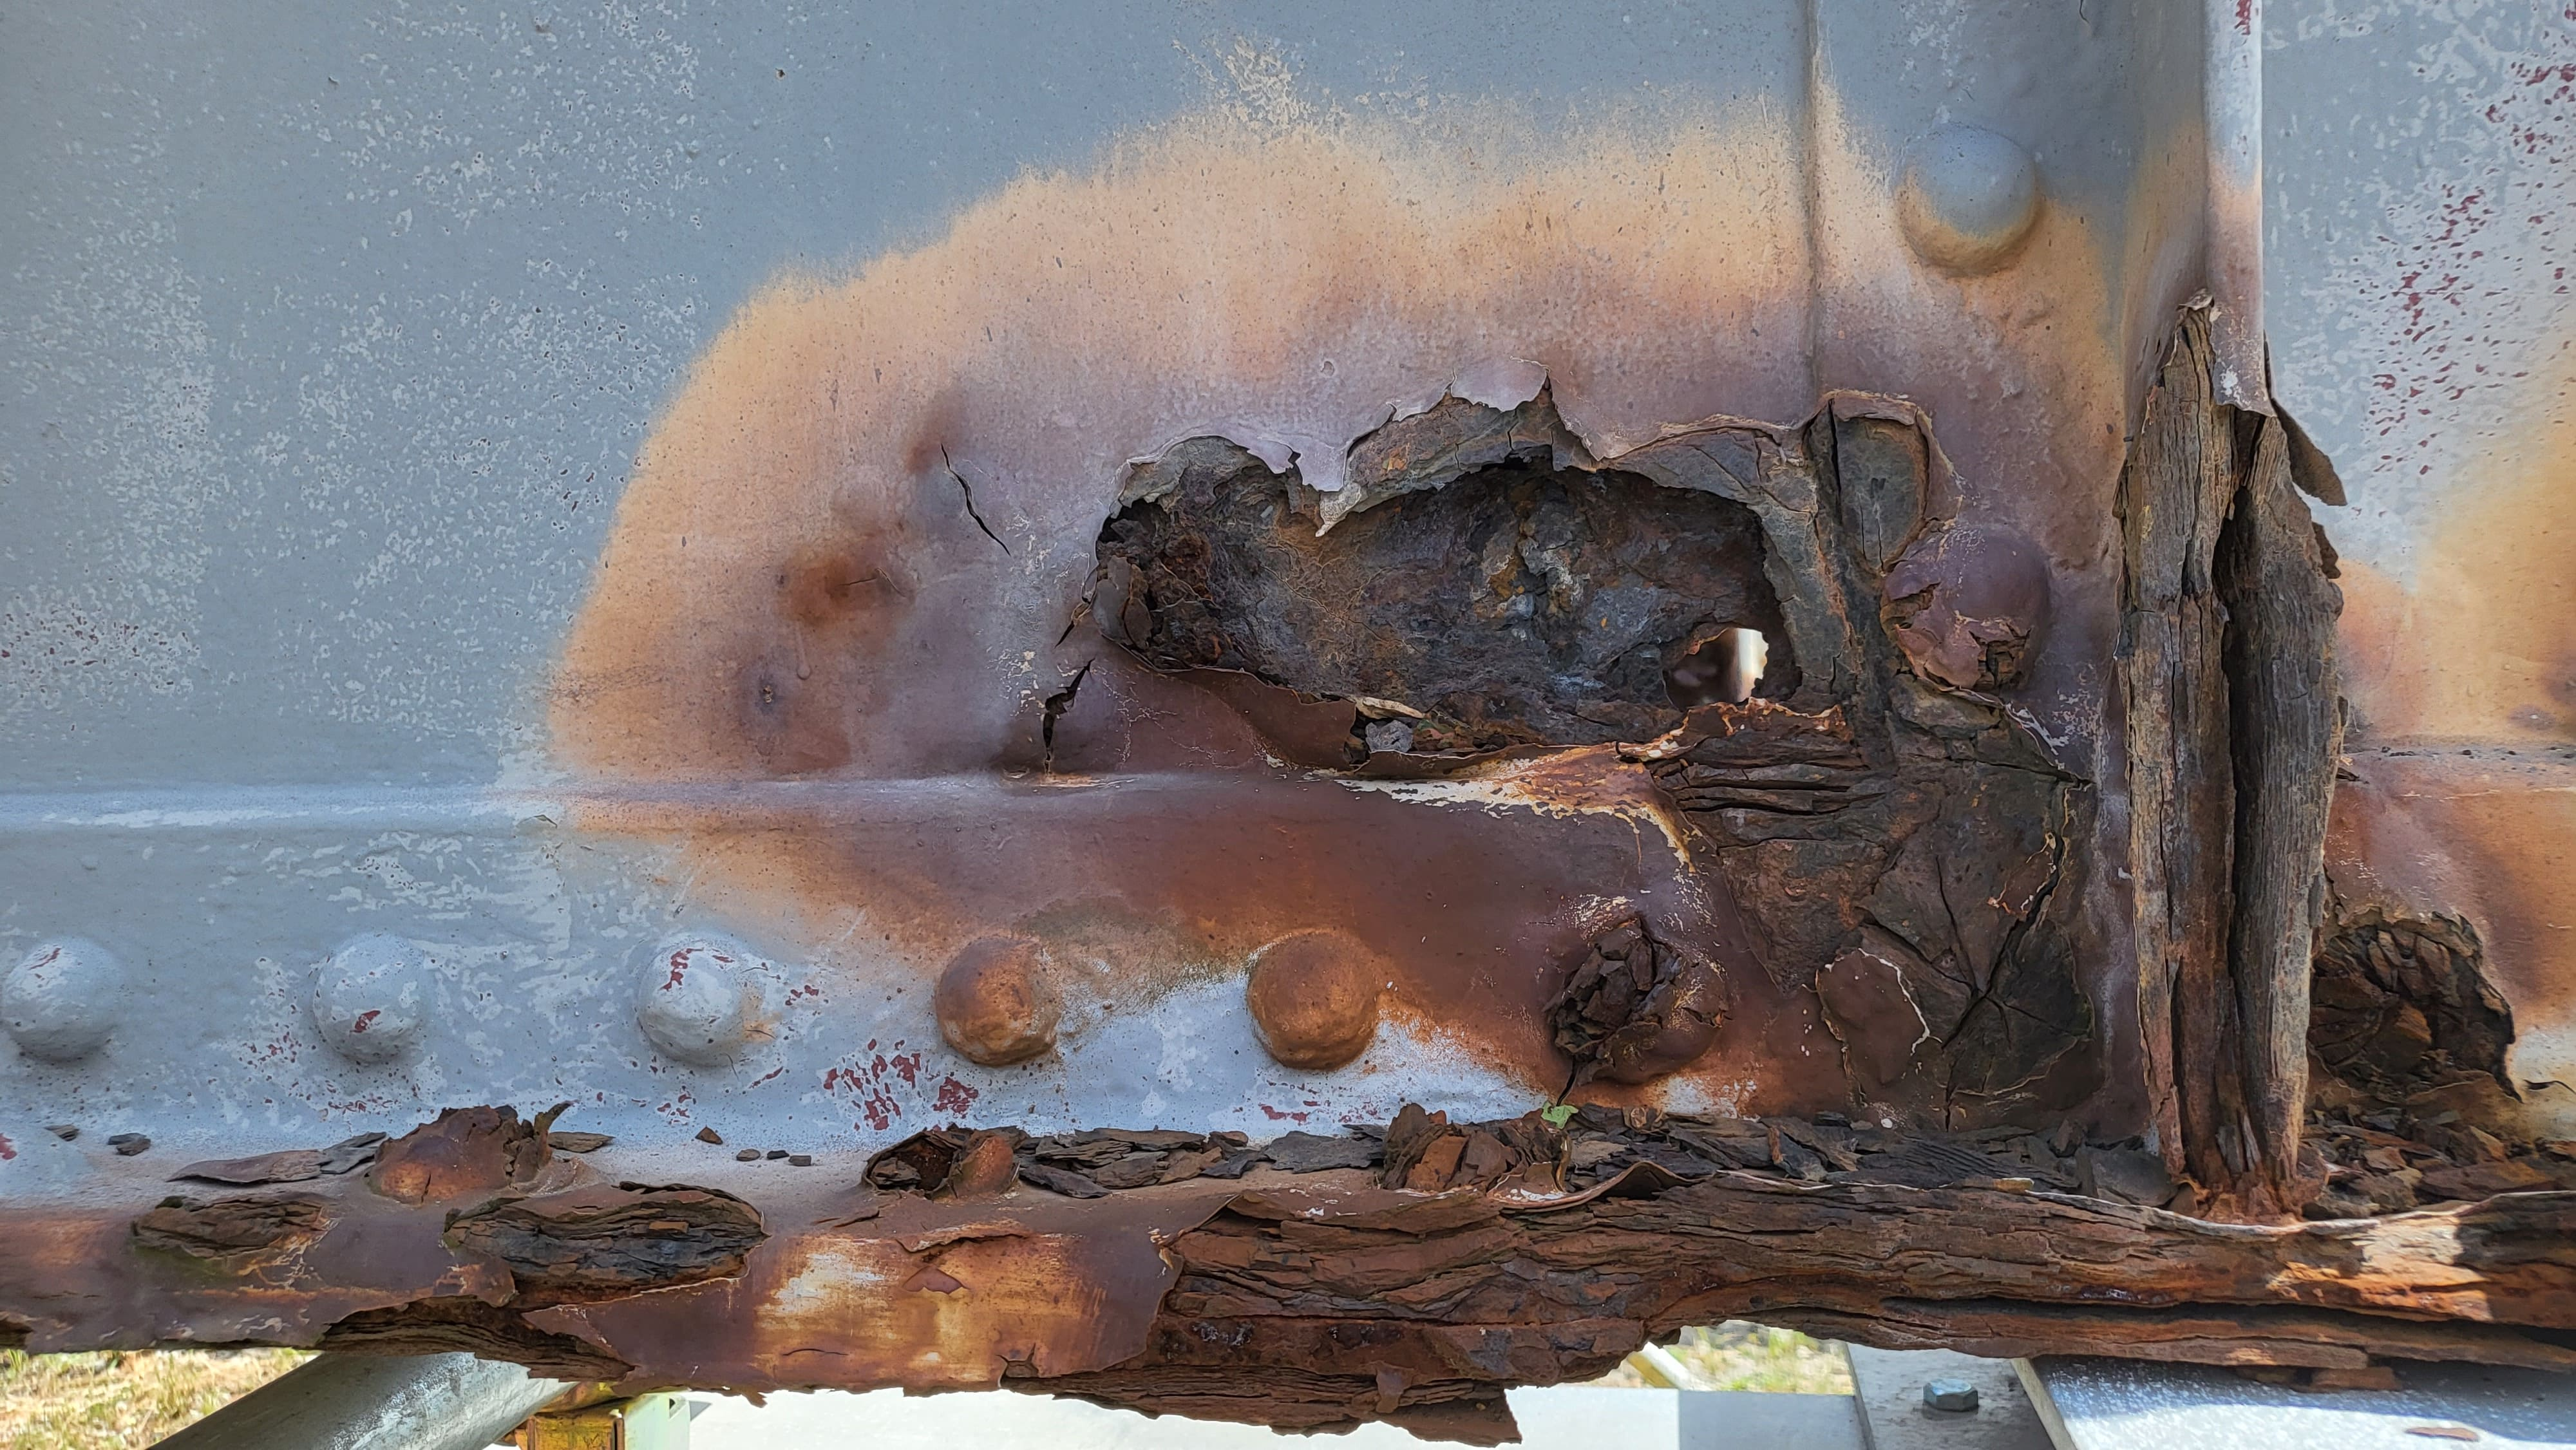
\includegraphics[width=\textwidth]{imgs/ch2/rivet-cor-1.jpg}%rivet-cor.png
        \caption{Corrosion of rivet}
        \label{fig-corriv}
    \end{subfigure}
    
    \begin{subfigure}[t]{0.85\linewidth}
        \centering
        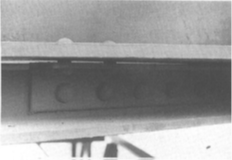
\includegraphics[width=\textwidth]{imgs/ch2/rivet-loss.png}
        \caption{Loosing of rivet}
        \label{fig-losriv}
    \end{subfigure}
    \caption{Aging condition of rivet}
\end{figure}


\begin{figure}
    \centering
    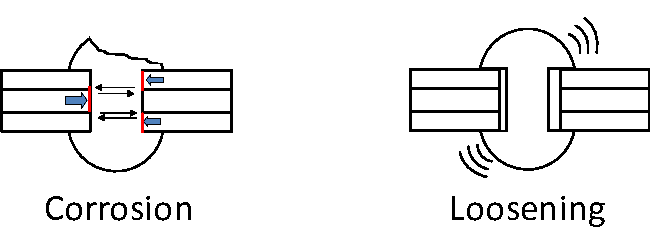
\includegraphics[width=0.8\textwidth]{imgs/ch2/rivet-issue.pdf}
    \caption{corrosion and loosing of aging rivet}
    \label{fig-rivetisu}
\end{figure}

\subsection{Mechanical behavior of riveted joint}

There are three types of resistance present in a riveted joint: friction, bearing, and shear. When it comes to force transfer utilizing a single rivet, there are two types: single-lap and double-lap as shown in Fig.\ref{fig-lapconnec}. Although an increase in the number of plates results in multi-sided shear, these two types are the fundamental structures of riveted joints in terms of force action. The forces transferred by the rivet only take into account the forces perpendicular to the rivet axis, such as direct tensile force. They do not consider the impact of axial tensile forces on the rivet head or its design. When two plates are joined by riveting, frictional forces transmit the load and restrict plate movement. This enhances the joint's strength, although it is not considered during the design process. Fig.\ref{fig-rsdisri} illustrates that the stress distribution, encompassing the rivet and the plate, is highly intricate. However, for practical purposes, it can be simplified into the following three types to facilitate design calculation for engineering.

\subsection{Design methods}

Riveted joints can be classified into approximately five types of failure model, depending on the strength of the rivet and the strength of the steel. Fig. \ref{fig-beafalmode} shows a fracture image of a single shear rivet. However, since the fracture of the main plate can be prevented by considering the placement of the rivets (model c--e), the shear strength of the rivets and the bearing strength are considered, and the strength of the bearing type connection is calculated using the smaller of the two values. 

\begin{figure}
    \centering
    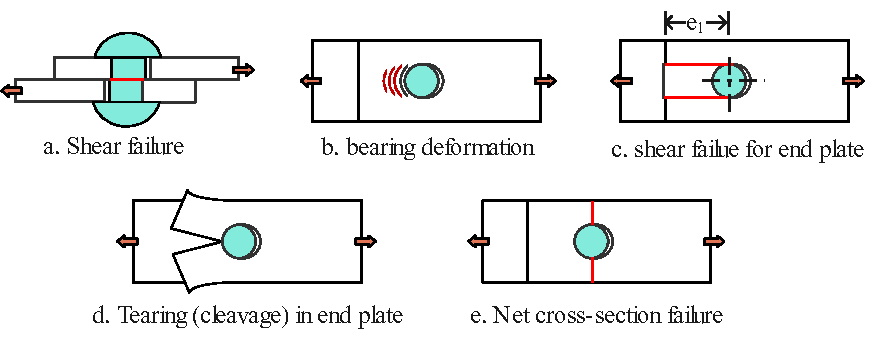
\includegraphics{imgs/ch2/failure-mode-bea.pdf}
    \caption{Failure mode of bearing type connection}
    \label{fig-beafalmode}
\end{figure}

For strength calculations of rivets, refer to Section \ref{secbc} on bearing type bolted connections, where national benchmarks use approximately the same calculation method for both rivets and bolts.


\subsection{Literature review}

Research has shown that riveted connections have been extensively studied in various countries in the past. However, most of the research has focused on the study of sound riveted connections, while studies on the deterioration of connections over time have evaluated the relationship between the structural integrity of the riveted structure and the service life, and have reported on the occurrence of damage and component performance degradation. The residual carrying capacity of corroded riveted beams and the estimation formulas for their carrying capacity have been specifically assessed through experiments and finite element analysis. However, these studies primarily focus on the residual carrying capacity of riveted connections and the residual performance of materials. There is less research on the repair and strengthening methods of riveted bridges, especially when rivets are replaced by high-strength bolts due to corrosion, and the changes in joint performance and load transfer mechanisms are not yet well understood.

\begin{figure}
    \centering
    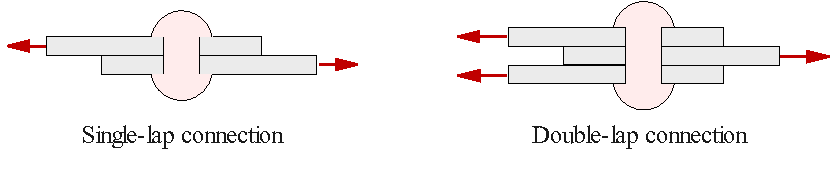
\includegraphics[width=0.85\textwidth]{imgs/ch2/lap-connec.pdf}
    \caption{Single \& Double lap connection}
    \label{fig-lapconnec}
\end{figure}


\begin{figure}
    \centering
    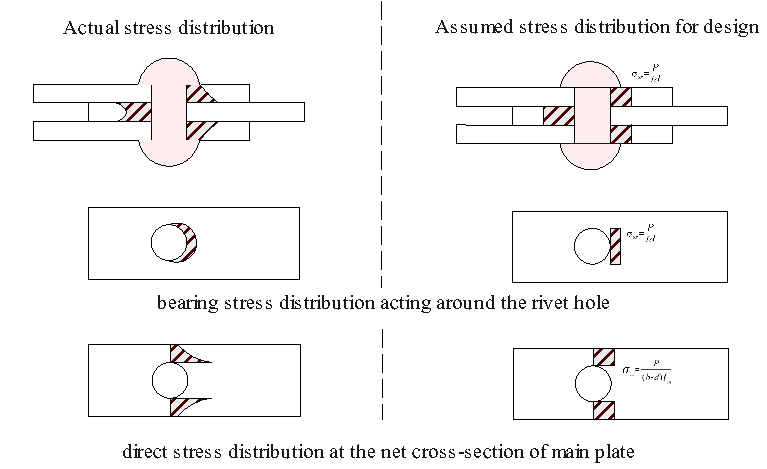
\includegraphics[width=0.85\textwidth]{imgs/ch2/bstressdistr-0.pdf}
    \caption{Stress distribution of double-lap riveted connection}
    \label{fig-rsdisri}
\end{figure}





\subsubsection{Assessment of riveted bridge: fatigue, strength, corrosion}
Extensive research on riveted joints has been conducted in numerous countries in the past. However, the majority of these studies focused on the examination of intact riveted joints. Haghani et al.\cite{haghani2012} conducted a comprehensive review of fatigue damage cases in over 100 bridges. Hołowaty et al. \cite{holowaty2022} examined the structural condition of 13 aged steel bridges constructed between 1873 and 1890, as well as 17 bridges spanning from 1907 to 1983.
Bacinskas et al. \cite{BACINSKAS2013136} conducted a study on the structural condition and behavior of a riveted steel truss bridge using full-scale static and dynamic testing. Aktan et al. \cite{aktan1994destructive} conducted a comprehensive series of nondestructive and destructive tests on two 80-year-old steel truss bridges that had been decommissioned, and the results show that, after completing each destructive test, no evidence of distortion or failure was found in the retrofitted connections. The effectiveness of the retrofit was demonstrated under the heavy concentrated loads experienced during destructive testing. Consequently, it can be deduced that similar bridges can be retrofitted to acceptable levels of safety with minimal effort and cost. Wang et al. \cite{wang2012} conducted a series of tests on an original steel angle obtained from a riveted truss Lanzhou Zhongshan Bridge, which was constructed in 1909. These tests examined the material mechanics, fracture behavior, and fatigue properties of the angle. Kossakowski \cite{kossakowski2013fatigue} presented the research findings on the fatigue strength of steel extracted from a railway bridge that had been in service for over a hundred years. The study focuses on analyzing and investigating the corrosion rate and assessing steel degradation. Małgorzata \cite{Skorupa2015InvestigationJoint} conducted experiments to investigate the load transfer mechanism of single-lap riveted joints and proposed a straightforward model to explain the transfer process. Gocál and Odrobiňák \cite{Gocal2020OnBridges} examines the influence of atmospheric corrosion on the load-carrying capacity of old riveted bridge structures. It analyzes the results and discusses the importance of long-term in situ corrosion measurements, as well as regular inspections for existing bridges. Reichle \cite{Reichle1999} analyzes the behavior of corroded rivets used in the connections of structural steel members. In particular, the material loss caused by corrosion is quantified using finite element analysis. And the findings of a parametric study and offers recommendations for deciding when to replace corroded rivets were presented. Zice \cite{Zice2023} conducted to investigate influences of the corrosion extent of rivet heads with artificial corrosion damage on the mechanical behaviour.

Numerous studies\cite{imam2008,Ryoichi2013,1987163,hisanori1991} have assessed the structural integrity of aging riveted connections in relation to their service life, and have reported on the correlation between the rate of damage and the decline in member performance. Through experiments and FEM analyzes\cite{nakata2016, Yurika2019,chen2022jp,cheniabse2022,Pipinato2014ResidualApproach,Bertolesi2021FatigueApproach}, the assessment of the remaining load bearing capacity of corroded riveted girders and the development of formulas for estimating said capacity have also been clarified. 

\subsubsection{Repair and reinforcement}
Lima et al.\cite{lima2008} presented the rehabilitation process of a century-old steel truss bridge with riveted connections in Canada. Kääriäinen \& Pulkkinen \cite{kaaria2002} documented the rehabilitation of the Tornionjoki steel truss bridge. Kimura et al.\cite{kimura2009} performed static loading tests to evaluate the strength of corroded rivet parts as well as the replaced parts using high-strength bolts. These components were obtained from a steel railway bridge that had been decommissioned, as well as from highway bridges. Siwowski \cite{siwowski2013} documented the rehabilitation of a continuous Warren-type steel truss bridge consisting of five spans, constructed in 1961. Gheitasi et al. \cite{Gheitasi2022} documented the rehabilitation of a historic steel truss bridge, which was 133 years old. The rehabilitation process involved partial dismantling, temporary relocation, and retrofitting, with a focus on various aspects of design and construction. Heydarinouri et al. \cite{Heydarinouri2021} presented a retrofit system that utilized pre-stressed CFRP bars to strengthen the double-angle connections between the stringers and floor beams of a riveted railway bridge in Switzerland, which had been in service for 92 years.



\subsection{Clamping force (Preload) of rivet}

When the heated rivet cools and hardens, the shrinkage of the rivet shaft introduces a significantly higher clamping force. In the past, there have been few studies to assess the clamping force of rivets due to limitations in measurement techniques. In the past, it was believed that the rivet would provide a clamping force equivalent to the yield point of the steel \cite{VanMaarschalkerwaart1982FatigueJoints}. However, subsequent experiments have shown that a clamping force of the yield point of the shaft part can be achieved by incorporating a relatively long rivet shaft ($>100 mm$). In contrast, when a short rivet shaft is present, the mean value of the clamping force introduced is lower, and the dispersion is also higher \cite{Zhou1994FatigueMembers, Baron1953TheJoints}. The deviation of the rivet head is believed to have a significant impact on the clamping force for short rivet axes.

Previous research findings \cite{Zhou1994FatigueMembers} indicate that the clamping force is dependent on the steel grade, particularly for rivets with a diameter of 24.5 mm. Therefore, Åkesson \cite{Akesson2010} refers to the nominal tensile stress caused by the clamping force in the axial section of the rivet as the clamping stress. The clamping stress to yield stress ratio of the rivet material was a crucial parameter in assessing the rivet clamping force. The average ratios were 0.61 and 0.77 for the rivet shaft lengths of 75 mm and 125 mm respectively. K{\"u}hn \cite{Kuhn2008AssessmentLife} have shown that the tightening force of st52 material rivets is lower than that of st37 material rivets. Heinemeyer \cite{Heinemeyer2011TheConnections} presents recent investigations on the impact of rivet head corrosion on the pre-stressing of the rivet, achieved through milling the rivet's head and conducting numerical simulations. It also presents fatigue tests that provide initial results for assessing the remaining lifespan of a riveted connection with reduced rivet stress.

The above mentioned previous studies mainly conducted tests in laboratory settings utilizing relatively long rivet shafts. Nevertheless, the actual clamping force introduced during riveting real bridges, particularly in-situ, differs to some extent from these experimental findings due to mistakes made during the riveting operation. A previous study8) removed rivets from real bridge girders and flanges to measure the residual rivet clamping force. Akesson \cite{Akesson2010} and Baron \& Larsson \cite{Baron1953TheJoints} reported comparable outcomes. Both sets of experimental data indicated that the length of the rivet shaft had a significant impact on the clamping force. Fig.\ref{fig-preload-rivet}  showed that a relatively long rivet shaft increased the average clamping force while decreasing its variance. Moreover, Leonetti \cite{Leonetti2020RivetBridges} also found that the number of plates also had an influence on the clamping force of the rivet. The misalignment of the holes of the plates has been reported to be caused by construction errors.

\begin{figure}
    \centering
    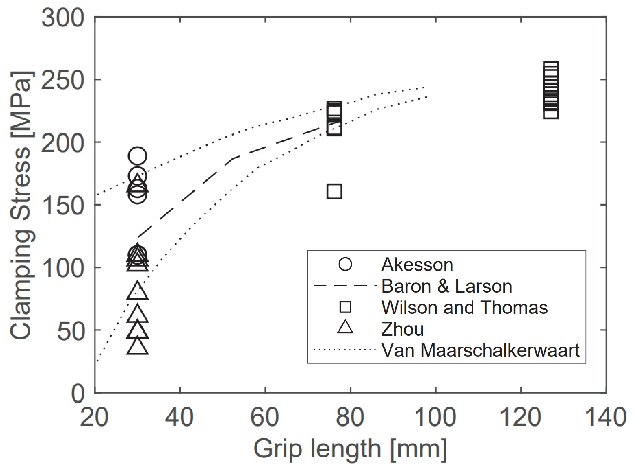
\includegraphics[width=0.8\textwidth]{imgs/ch2/preload-rivet.pdf}
    \caption[The variability of the clamping stress as a function of the grip length for carbon steels.]{The variability of the clamping stress as a function of the grip length for carbon steels. (figure cite from \cite{Leonetti2020RivetBridges}, experimental data from Åkesson \cite{Akesson2010},Wilson and Thomas \cite{Wilson1938FatigueJoints}, and Zhou \cite{Zhou1994FatigueMembers}. Also the average trend from Baron \& Larson \cite{Baron1953TheJoints}, and upper and lower bounds from van Maarschalkerwaart \cite{VanMaarschalkerwaart1982FatigueJoints} are reported.)}
    \label{fig-preload-rivet}
\end{figure}


\subsection{Remaining issue}
However, the primary focus of these studies is on the residual carrying capacity of riveted connections and the residual performance of materials. Insufficient research has been conducted on the repair and strengthening methods of riveted bridges, especially in cases where corrosion leads to the substitution of rivets with high-strength bolts, resulting in limited understanding of the alterations in joint performance and load transfer mechanisms. Steel riveted bridges hold significant cultural and historical value as a part of our constructive heritage from the previous century. Numerous iron and steel riveted bridges are of historical importance, requiring restoration and preservation, and are currently operational.

\section{Friction type bolted connection}

\subsection{Background}

Friction-type High-strength bolt connections have been widely used in building steel structures recently due to their ease of installation, higher bearing capacity, and superior anti-fatigue performance. The high-strength bolt connection can be classified into bearing type and friction type based on the difference in force transmission patterns as shown in \ref{fig-fricandbearing}. In the case of the bearing type, the connection's bearing capacity depends on the resistance of the hole wall and the shear resistance of the bolts. In the case of the friction type, the force is transmitted through friction between the faying surfaces of the plates. The resistance of the bearing type connection is typically higher than that of the friction type. However, the bearing type connection is not directly suitable for fatigue and dynamic loads.

\begin{figure}
    \centering
    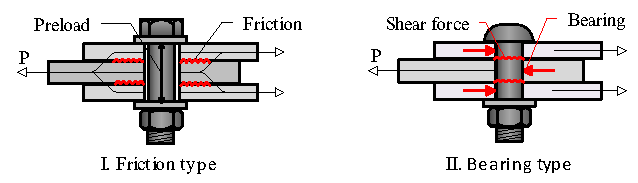
\includegraphics[width=0.85\textwidth]{imgs/ch2/fricandbearing.pdf}
    \caption{Schematic of load transmit mechanism of friction-type and bearing-type bolted connection}
    \label{fig-fricandbearing}
\end{figure}

The mechanical properties of bolted joints have a direct impact on their load-bearing capacity. The spacing, strength, and stress state of bolts all play a crucial role in determining the mechanical properties of high-strength bolted joints. Extensive research has been conducted over the years to investigate the various factors that affect these properties \cite{peng2015,Lyu2019NumericalSteels,Brian1996EdgeOcnnections,wang2020interface,hirashima2004experimental}. This research has helped identify ways to optimize the performance of bolted joints, ensuring the safety and longevity of structures in diverse applications. Understanding the factors that influence these properties enables engineers and designers to make informed decisions regarding material selection and structural design to meet specific performance requirements.

The construction of new bridges often entails several design challenges. Among these challenges is the requirement to enhance the strength of bridge components to withstand increased external live loads, without necessitating a larger overall structure. This necessity for adjustments has gained prominence in recent years, coinciding with the growing utilization of high-strength steels in bridge construction.

To fulfill this requirement, the bolted joints within the steel bridge structure must be engineered to endure the augmented strength of the steel components. However, the strength of friction-type joints is influenced by two primary factors: the quantity of bolts employed and the slip coefficient. 

Increasing the number of bolts is a simple and effective measure. However, an increase in the number of bolts means that the size of the joint will become larger, resulting in added weight. Large joints bring about several disadvantages, such as decreased load-carrying capacity with increasing side length of the joint. Additionally, an increase in the number of bolts complicates the management and maintenance of the bolt group, thereby increasing the maintenance costs of the bridge.

\subsection{Design methods}

%各国设计标准对于slip resistance的计算方法都一样可以通过式子-ch2fs计算得出。然而,对于一些折减系数的定义各国标准略有不同,例如对于孔大小的折减等,这里就不做探讨了。

\begin{equation} \label{ch2fs}
    F_s=\mu m N_0
\end{equation}

where, m is the number of friction planes, $\mu$ is the slip coefficient of faying surface, $N_0$ is the initial preload before loading, $n_0$ also can be calculated by $0.7f_{ub}A_s$

\subsection{Long bolted joint}
As a joint length increases, problems arise when using  long or large bolted joints. First, owing to the presence of secondary members in the vicinity of the joint (e.g., stiffener and diaphragm), excessively long joints can interfere with secondary members. Therefore, it is necessary to shorten the length of the joint while maintaining design strength. Typically, a slip-critical joint combined with a weld is used to satisfy the design strength requirements of a joint. Previous studies have demonstrated that slip-critical bolted joints combined with welds are reliable and feasible \cite{solodov2021,Thomas2000,Chang2019361,KHANDEL2022107036}. Combinations of welded--bolted connections are widely used in steel structures. However, some environments, such as those offering insufficient space or requiring work at height, are not conducive to welding during onsite bridge construction. Welding also destroys the original coating of steel parts, which necessitates repainting the joints. As a result, the construction of combined welded--bolted connections is very difficult for steel bridge joints that require onsite joining. Appropriate methods are required to shorten the bolted joint without reducing its strength. \par

Second, as the length of the joint (defined as the spacing between the first and last fasteners in a joint) increases, the resistance that can bolt provide decreases to a value lower than the slip strength because the distribution of the bolts inside the joint becomes uneven. As the joint length increases with an increasing number of bolts in a line, the differential deformations in the main plate causes shear failure at the end bolts before all bolts can develop their full shearing strength. This ''unbuttoning'' phenomenon has been observed for all types of fasteners including rivets \cite{fisher1965behavior}. Bendigo et al.\cite{bendigo1963long} concluded that for longer connections, end bolts are sheared before all the bolts can develop their full shear strength. For short connections, the average shear stress is approximately 85\% that of a single bolt; however, for a 52.5 inch long connection, bolts only develop 60\% of their strength. Kamei et al. \cite{KAMEI2000} also showed that the serviceability limit strength decreases by approximately 2.5 $\%$ for each additional row.  Tan et al.\cite{Tan2022} considered that when the number of rows of bolts is more than 5, the force transmission ratio of the end bolt is 0.389.

Owing to the above issues, specifications for long-bolted joints, such as AASHTO, Eurocode, as well as Japanese and Chinese, all provide a reduction factor based on the length of the bolted joint\cite{AASHTO2020,eccs1985,isohtb,eurocode3-21,douji2017}. Furthermore, owing to uneven load sharing, the bolts cannot simultaneously fracture, and the ultimate limit bearing capacity decreases \cite{Takai2021BoltUnbuttoning,Peng2013FeaDimensions,peng2010,longstainless2022}. 

The European Convention for Constructional Steelwork (ECCS), and ISO/TC specify that the resistance should be reduced by a factor of $\beta_{rd}$ when the spacing between the first and last bolt in a joint is larger than 15d as shown in Eq.\ref{ch2eq1} \cite{eccs1985,isohtb}. AASHTO \cite{AASHTO2020} provides the nominal shear resistance of bolts in joints longer than 38.0 in. must be reduced by an additional factor of 0.83 or 0.75/0.9\par

\begin{equation}
    \beta_{rd} = \begin{cases}1 & (L \leq 15 d) \\ 1.08-L /(200 d) & (15 d<L \leq 65 d) \\ 0.75 & (65 d<L)\end{cases}
    \label{ch2eq1}
\end{equation}

Eurocode 3 (EN 1993-1-8:2005) \cite{eurocode3-21} provisions that where the distance $L_j$ between the centers of the end fasteners in a joint, measured in the direction of force transfer is more than 15d, the design shear resistance of all the fasteners should be reduced by multiplying it by a reduction factor $\beta_{Lf}$:
\begin{equation}
    \beta_{Lf}=1-\frac{L_j - 15d}{200d}
\end{equation}

Japanese Specification for Highway Bridge (JSHB) \cite{douji2017} published by Japan Road Association states that when the number of row exceeds 8 in bolted joint, a reduction factor must be applied to the slip strength, as shown in Table \ref{tab-jpredu}.
\begin{table}[h]
    \centering
    \caption{Reduction of slip strength of bolted joint of JSHB-JRA}
    \begin{tabular}{cccccc}
    \toprule
        Number of Row &  8 & 9 & 10 & 11 & 12 \\ \midrule
        Reduction factor & 1.00 & 0.98 & 0.96 & 0.94 & 0.92 \\ \bottomrule
    \end{tabular}
    \label{tab-jpredu}
\end{table}

Furthermore, due to the non-uniformity of load distribution, the bolts are unable to fracture simultaneously, consequently leading to a reduction in the ultimate limit bearing capacity.\cite{Takai2021BoltUnbuttoning,Peng2013FeaDimensions,peng2010}.

Considering the installation space requirements and strength problems associated with long-bolted joints, a rational compact joint must be developed to allow the use of fewer bolts to transmit more load, which could also improve the serviceability limit capacity of the joints.

\subsection{Technical Problem} %%todo , add the long bolted joint figure.
Problems arise when utilizing long or large friction-type bolted joints as the joint length increases. Firstly, these excessively long bolted joints can cause interference with secondary members, such as stiffeners and diaphragms, located in close proximity to the joint as shown in Fig. \ref{fig-boxhsbinter}. Therefore, it becomes necessary to reduce the joint length while maintaining the design strength. Typically, a friction-type bolted joint combined with a weld is employed to meet the design strength requirements of a joint. Previous studies have demonstrated the reliability and feasibility of friction-type bolted joints combined with welds \cite{solodov2021,Thomas2000,Chang2019361,KHANDEL2022107036}. Combinations of welded-bolted connections are sometimes utilized in steel structures to improve their strength. However, However, this combination methods is inefficient in terms of load bearing capacity enhancement, also the certain environments, such as those with limited space or requiring work at height, are not conducive to onsite welding during bridge construction. Additionally, welding destroys the original coating of steel parts, necessitating reapplication of the protective paint to the joints. Consequently, the construction of combined welded-bolted connections for steel bridge joints that require onsite joining becomes highly challenging. Thus, suitable approaches are required to reduce the length of bolted joints without compromising their strength.

\begin{figure}[htbp]
    \centering
    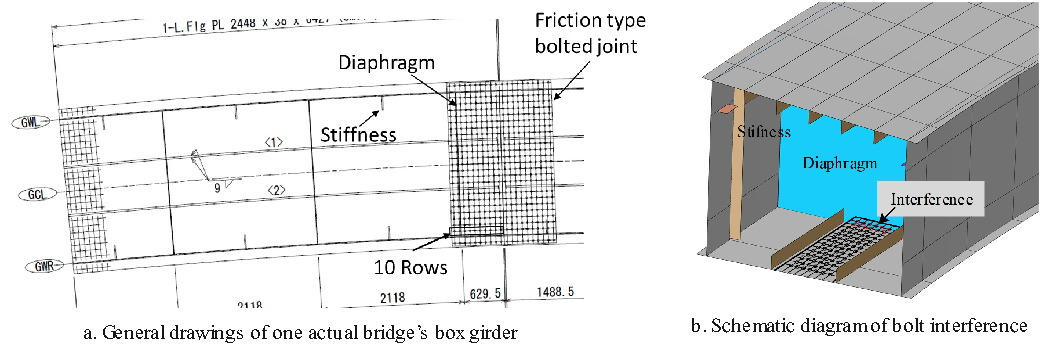
\includegraphics[width=1\linewidth]{imgs//ch2/boxhsbinter.pdf}
    \caption{Actual engineer case of the need of hybrid joint: the joint of box girder}
    \label{fig-boxhsbinter}
\end{figure}

Second, as the length of the joint (defined as the spacing between the first and last fasteners in a joint) increases, the resistance that can bolt provide decreases to a value lower than the slip strength because the distribution of the bolts inside the joint becomes uneven. As the joint length increases with an increasing number of bolts in a line, the differential deformations in the main plate causes shear failure at the end bolts before all bolts can develop their full shearing strength. This "unbuttoning" phenomenon has been observed for all types of fasteners including rivets \cite{fisher1965behavior}. Bendigo et al.\cite{bendigo1963long} concluded that for longer connections, end bolts are sheared before all the bolts can develop their full shear strength. For short connections, the average shear stress is approximately 85\% that of a single bolt; however, for a 52.5 inch long connection, bolts only develop 60\% of their strength. Kamei et al. \cite{KAMEI2000} also showed that the serviceability limit strength decreases by approximately 2.5 $\%$ for each additional row.  Tan et al.\cite{Tan2022} considered that when the number of rows of bolts is more than 5, the force transmission ratio of the end bolt is 0.389.

Owing to the above issues, specifications for long-bolted joints, such as AASHTO \cite{AASHTO2020}, Eurocode3 \cite{eurocode3-21}, as well as Japanese and Chinese, all provide a reduction factor based on the length of the bolted joint \cite{eccs1985,isohtb,douji2017}. Furthermore, owing to uneven load sharing, the bolts cannot simultaneously fracture, and the ultimate limit bearing capacity decreases \cite{Takai2021BoltUnbuttoning,Peng2013FeaDimensions,peng2010,longstainless2022}. 

Considering the installation space requirements and strength problems associated with long-bolted joints, a rational compact joint must be developed to allow the use of fewer bolts to transmit more load, which could also improve the service limit capacity of the joints.

\section{Bearing type bolted connection} \label{secbc}

\subsection{Background}

The HSB bearing type connection is a connection method based on the idea that, as in the case of friction connections, a preload is usually introduced into the bolt and frictional resistance is used for normal loads, while shear resistance of the bolt shaft and bearing resistance of the base metal and the connecting plate are expected for emergency loads, such as an earthquake \cite{rivet1977}. There are four types of bolt that can be used for support connections: those with a shape similar to that of a friction connection, those with an interference fit (hammered-in type), and the resin-injected bolt or the mechanical bolt-rivet. These bolts are characterised by their method of load transmission, relying primarily on bearing against the sides of holes in the fasteners and friction to transmit forces in a hybrid manner.

Bearing bolts operate on a simple mechanical principle: When a load is applied to the connected structure, it induces direct bearing forces on the bolt shank. These forces, in turn, are transferred to the material surrounding the bolt holes by bearing stress. These bolts are not designed to be preloaded; they operate as soon as the load causes the connected elements to press against the bolt. For optimum performance, the hole diameter is made slightly larger than the diameter of the bolt for ease of installation; however, this clearance must be minimal to maintain load transfer without yielding or excessive deformation. ASTM standards \cite{ASTM-bolt} and others provide guidelines for these tolerances to ensure proper function.

In recent years, the use of bearing type connections has been reported\cite{morikawa2002} in cases where the required performance of the friction faying surface is not satisfied, such as in the case of a reinforce method for fatigue cracks at the corner of steel piers, but the number of applications to actual bridge main members is extremely small. 

Although the bearing-type connection can offer much higher strength compared to the friction-type connection \cite{Li2020bbolt,perry1981bearing,kim1999bearing}, it also faces a series of issues such as poor construction performance and high precision requirements, their application comes with inherent challenges. First, the precise required tolerances between the bolts and the holes. Since load transfer depends on the bearing of the bolt against the edge of the hole, any significant misalignment or incorrect size can lead to reduced load capacity or even structural failure. Furthermore, these connections are susceptible to slipping when exposed to dynamic or cyclic loads, necessitating careful consideration of the slip coefficients of the connected materials and the potential for fatigue.

Moreover, in environments prone to corrosion or where long-term durability is a concern, protective measures must be implemented to preserve the integrity of the bearing-type bolts. Regular inspections are vital to detect any signs of wear, corrosion, or loosening that could compromise the connection's integrity.

In summary, it can be expected that in the future bearing type bolts will be a fundamental element in the design of steel structures, offering a balance between strength, ease of assembly and cost effectiveness.

\subsection{Design resistance}

\subsubsection{Bearing resistance at fastener hole}

In Japan, the latest 2017 edition of the \ac{JSHB} by \ac{JRA} \cite{douji2017} states that bearing type connections can be designed according to the service limit, and the serviceability limit state is determined by checking the shear yield strength of the bolt shaft, and the bearing strength of the main plate.

The bearing strength by JSHB shall be taken as:

\begin{equation}
    F_{b,JSHB} = 1.7 f_y dt
\end{equation}

On the other hand, \ac{JSRS} by \ac{RTRI} \cite{rtri2009Design} states that the area subjected to bearing stresses is less likely to experience plastic flow with yielding due to the surrounding restraints, and that strength above the yield point can be expected. The bearing strength is 50\% above the yield point of the jointed material, as shown in Eq. \ref{eqfbjsrs}.

\begin{equation}\label{eqfbjsrs}
    F_{b,JSRS} = 1.5 f_y dt
\end{equation}


Where, $d$ is nominal diameter of the bolt, $t$ is thickness of the main plate, $f_y$ is the yield strength for main plate.

AASHTO MBE \cite{aashtombe2018Manual} states that the design of rivets can be directly referred to AASHTO LRFD BDS for bearing type connection, and the specifications states that the effective bearing area $A_{b}$ of a fastener is its diameter $d$ multiplied by the thickness of the main plate $t$ on which it rests, and should be designed for strength limit states。 The bearing strengths are as follows:

AASHTO LRFD BDS 9th editions:

When clear distance between fastener hole $L_c$ is not less than 2d, and with a clear end distance $e_1$ not less than 2.0d:

\begin{equation}
    F_{b,AASHTO} = 2.4dtf_u
\end{equation}

When fastener spacing $L_c$ is less than 2d, and with a clear end distance $e_1$ less than 2.0d:
\begin{equation}
    F_{b,AASHTO} = 1.2L_ctf_u
\end{equation}

Where, $f_u$ is tensile strength stress for the main plate, $L_c$ is clear distance between fastener holes, $e_1$ is the distance between end of plate and the end fastener hole center.

Eurocode 3 \cite{eurocode3-21} states that the bearing type connection (Category A) should be design as ultimate limit state \cite{ec1993-1-1-2020} and can be used without regard to the application of preload and the requirements of the joint faying surface, and that the bearing strength of the bearing type connection can be calculated in accordance with the following formula:

\begin{equation}
    F_{b,EC3} = k_m\alpha_bf_udt
\end{equation}

Where, for steel grades equal to or higher than S460 $k_m$ is 0.9, otherwise $k_m$ is 1

- for end bolts: $\quad \alpha_{\mathrm{b}}=\min \left(\frac{e_1}{d_0} ; 3 \frac{f_{\mathrm{ub}}}{f_{\mathrm{u}}} ; 3\right)$

- for inner bolts: $\quad \alpha_{\mathrm{b}}=\min \left(\frac{p_1}{d_0}-\frac{1}{2} ; 3 \frac{f_{\mathrm{ub}}}{f_{\mathrm{u}}} ; 3\right)$

The Chinese national standard of steel structure \ac{CSSS} GB50017-2017 \cite{gb50017-2017} stipulates that the SLS of bearing type connection can be used in accordance with the friction type connection calculation, while the bearing strength $F_{b,CS}$ is stipulated as the strength limit state, which can be obtained by the following formula calculation:

\begin{equation}
    F_{b,CS}=1.26 f_u dt
\end{equation}

\subsubsection{Shear resistance at fastener shaft}

The \ac{JSHB} stipulates that the shear strength of the bearing type connection for the main plate can be designed as the Serviceability limit strength and Ultimate limit strength respectively, which are calculated by the following formula.

For the SLS:

\begin{equation}
    F_{vf,JSHB,SLS} = f_{yf}/\sqrt{3}A_s
\end{equation}

For the ULS:

\begin{equation}
    F_{vf,JSHB,ULS} = f_{uf}/\sqrt{3}A_s
\end{equation}


Where, $f_{yf}$ is the yield strength stress of fastener. $f_{uf}$ is the ultimate strength stress of fastener. $A_s$ is the effective area of fastener shaft, can be calculated as $A_s = \frac{\pi d^2}{4}$.

\ac{AASHTO} \cite{AASHTO2020} state that the nominal shear resistance of a HSB at ultimate limit state in joints whose length between extreme fasteners measured parallel to the line of action of the force is less than or equal to 38.0 in. And the nominal shear resistance of bolts in joints longer than 38.0 in. must be further reduced by an additional factor of 0.83 or0.75/0.90.
The shear resistance at fastener shaft can be calculate as following formula:

- Where threads are excluded from the shear plane:

\begin{equation}
    F_{vf,AASHTO} = 0.56f_{uf}A_s
\end{equation}

- Where threads are include in the shear plane:

\begin{equation}
    F_{vf,AASHTO} = 0.45f_{uf}A_s
\end{equation}

Eurocode 3 states that the  shear resistance at fastener shaft can be calculate as following formula:

- Where threads are excluded from the shear plane:
\begin{equation}
    F_{vf,EC3} = \alpha_v f_{uf}A_s
\end{equation}

- Where threads are excluded from the shear plane (Rivets are also calculated according to this formula):
\begin{equation}
    F_{vf,EC3} = 0.6 f_{uf}A_s
\end{equation}

Where, For property of the bolt is classes 4.6, 5.6 and 8.8, $\alpha_v$ is 0.6. For property of the bolt is classes 4.8, 5.8 and 10.9, $\alpha_v$ is 0.5.

Chinese standrad \ac{CSSS} states that the  shear resistance at fastener shaft can be calculate as following formula:

\begin{equation}
    F_{vf,CSSS} = 0.3 f_{uf}A_s
\end{equation}

Where, when the bolt class is lower or equal to the class 8.8, the shear resistance should be taken as $0.4f_{uf}A_s$


\subsubsection{Shear resistance at main plate}

In addition to calculating the above two types of resistance of bearing, the general calculation of load bearing strength should also confirm that the main plate will not occur in the end shear failure, the main plate should be prevented from occurring in Fig. \ref{fig-beafalmode}, such as c. end shear, and d. end tearing failure occurs.

The \ac{AIJ} \cite{2012AIJStructures} provides two methods for calculating the edge shear resistance $F_{vp,AIJ-1}$ : one is to calculate the shear plane based on the effective cross-sectional area $A_{vp}$, and the other is to calculate it based on the equivalent shear cross-sectional area $A_{vp2}$.

- For the effective cross-sectional area:

\begin{equation}
    F_{vp1,AIJ-ef} = 0.5 A_{vp}f_u
\end{equation}
Where, 

\begin{equation}
    A_{vp} = 2 {e_1 + (n-1)p}t
\end{equation}

- For the equivalent cross-sectional area:

\begin{equation}
    F_{vp1,AIJ-2} = A_{vp2}\sqrt{3}f_u
\end{equation}

Where,

\begin{equation}
A_{vp2}=2\left[\left\{e_1-\frac{\sqrt{2}-1}{2} d\right\}+\left\{p_1+(\sqrt{2}-1) d\right\}(n-1)\right] t
\end{equation}

On the other hand, Kulak \cite{Kulak1988guide} states that the maximum bearing capacity can be expressed by the following Eq. \ref{eqfkulak} based on the experimental results of end-failure joints. The reason why an upper limit is specified for the maximum proof stress is that the failure mode is not end failure (Fig. \ref{fig-beafalmode}-c) but bearing failure (Fig. \ref{fig-beafalmode}-b) when the load exceeds this limit.

\begin{equation}\label{eqfkulak}
    F_{vp,kulak}=2t(e_1-2/d)(0.7f_u)
\end{equation}

\begin{equation}
    F_{b,kulak}=3dtf_fu
\end{equation}

The definition of each symbol for the joint is shown in the following Fig. \ref{fig-symbol}.

\begin{figure}
    \centering
    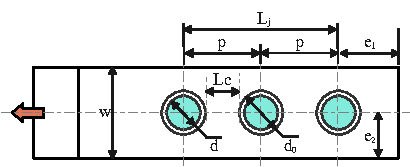
\includegraphics[width=0.7\linewidth]{imgs//ch2/symbol.pdf}
    \caption{The use of the symbols}
    \label{fig-symbol}
\end{figure}

Eurocode 3 also state that the block tearing should be avoided. For a bolt group where the tension stress on the tension area is uniform as shown in Fig. \ref{ch2figeu5-13}, the design block tearing resistance $v_{eff,1}$ should be taken as:

\begin{equation}
    v=[A_{nt}f_u+min(\frac{A_{gv}f_y}{\sqrt{3}}; \frac{A_{nv}f_u}{\sqrt{3}})]/\gamma_{M2}
\end{equation}

where, $A_{nt}$ is the net area subjected to tension, $A_{gv}$ is the gross area subjected to shear, $A_{nv}$ is the net area subjected to shear.

\begin{figure}
    \centering
    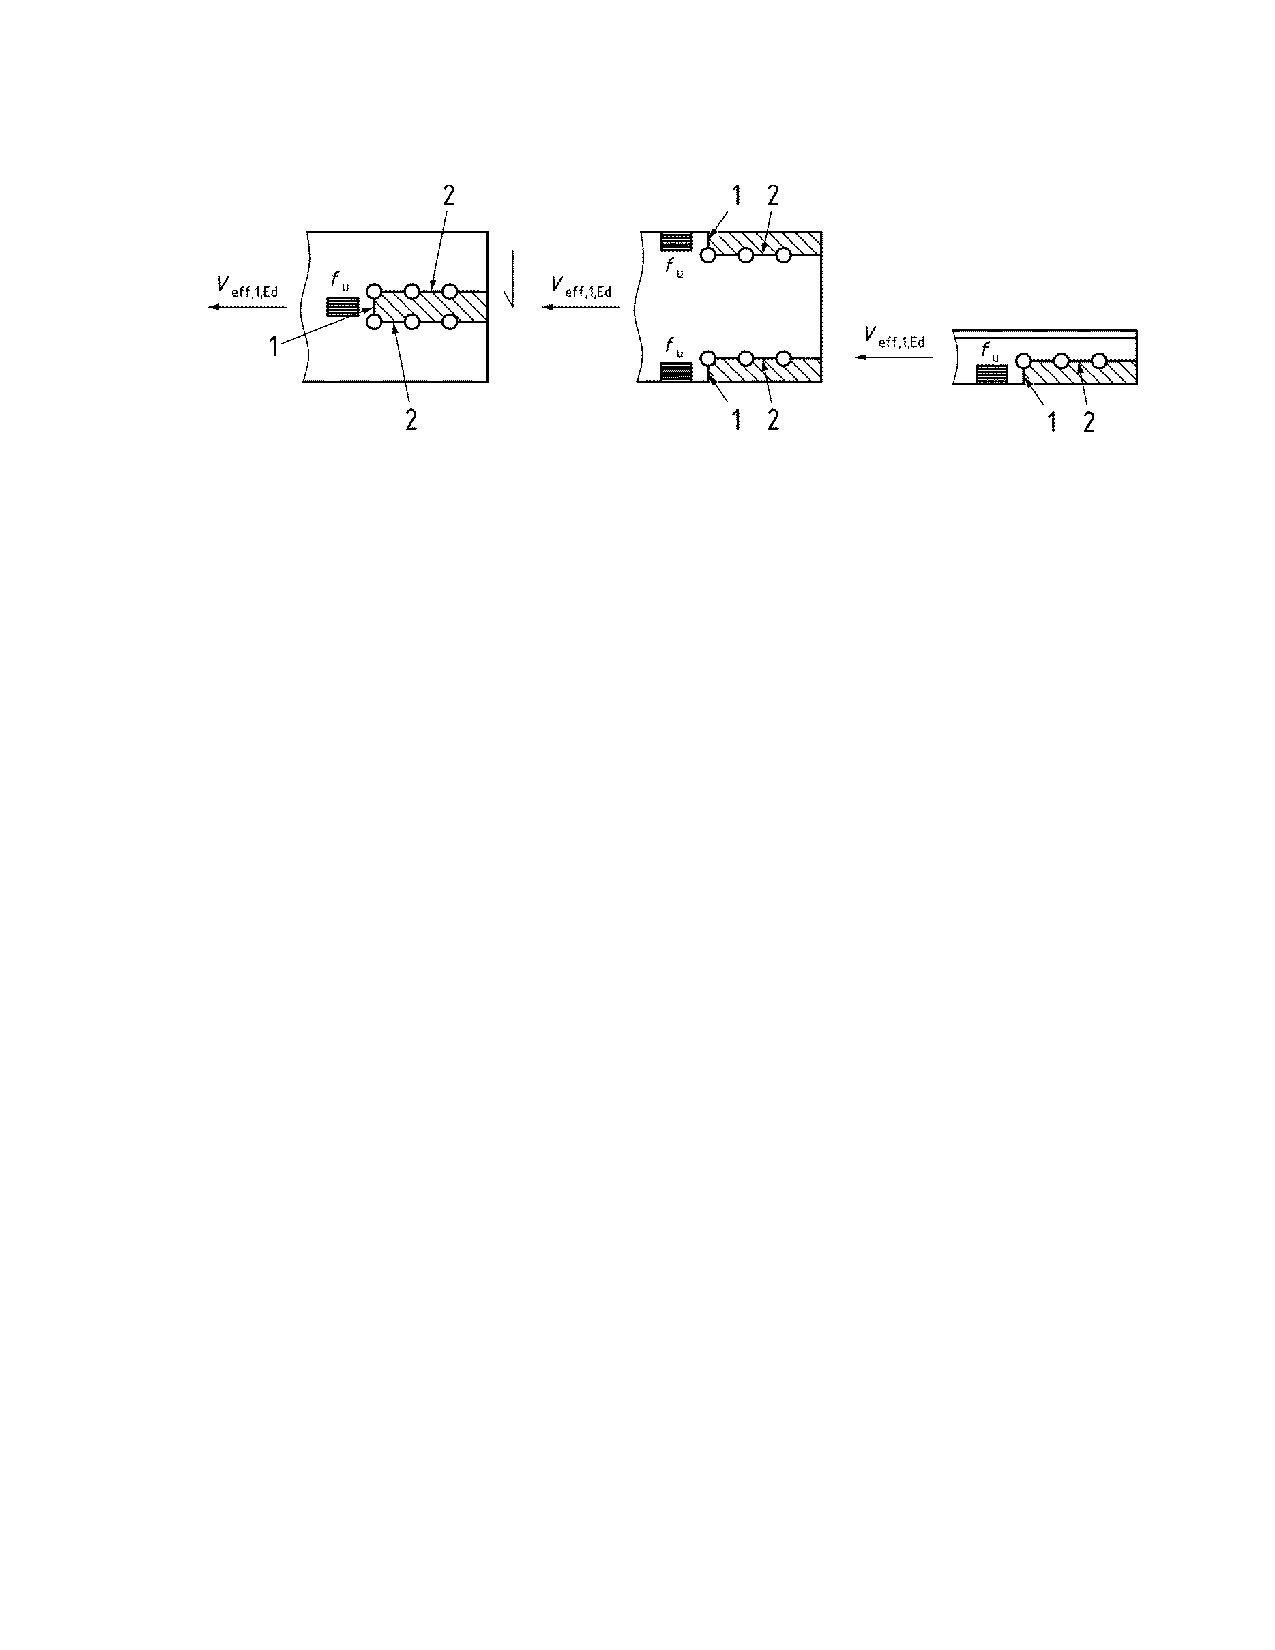
\includegraphics[width=0.7\linewidth]{imgs/ch2/ch2figeu5-13.pdf}
    \caption{The use of the symbols}
    \label{ch2figeu5-13}
\end{figure}


\subsection{Interference fit bolt}

A specialized high-strength bolt for bearing-type connection is present, the bolt have rib around the bolt shaft, the outermost diameter include rib should be over than the bolt hole, so when hanmer into the bolt, the rib will have occur plastic deformation and general interference fit effect, hereafter known as the Interference fit bolt \cite{Kulak1988guide,bolt-bearing,Chen2023MechanicalConnections} as shown in Fig. \ref{fig-onebbolt}. The B10T grade interference fit bolts were used (courtesy of Kobelco Bolt, Ltd.) and meets the strength requirements of an F10T bolt according to the JIS-B1186 standard \cite{jis2018JIS}, which is equivalent to ASTM-A490 \cite{ASTM-bolt} \& Grade 10.9 \cite{ISO-bolt} and possesses the unique feature of an axially ribbed shank. When the bolt is hammered into a hole, the rib undergoes plastic deformation to ensure a tight fit and prevents excessive slipping. Interference fitting bolts are used to retrofit steel bridge piers that have fatigue damage or corrosion by attaching the patch plate \cite{Anami-bbolt-ate}. This is because initial imperfections or corrosion leads to uneven steel plate surfaces, making it impossible for the patch plate of the friction type bolted connection to effectively contact the steel surface and transmit force. And Interference fit bolts also can reduce the fatigue damage in bolt holes, and increasing their fatigue strength \cite{Guo20205}. However, interference fit bolts are rarely used on other bridge parts due to their stringent installation requirements. 

\begin{figure}
    \centering
    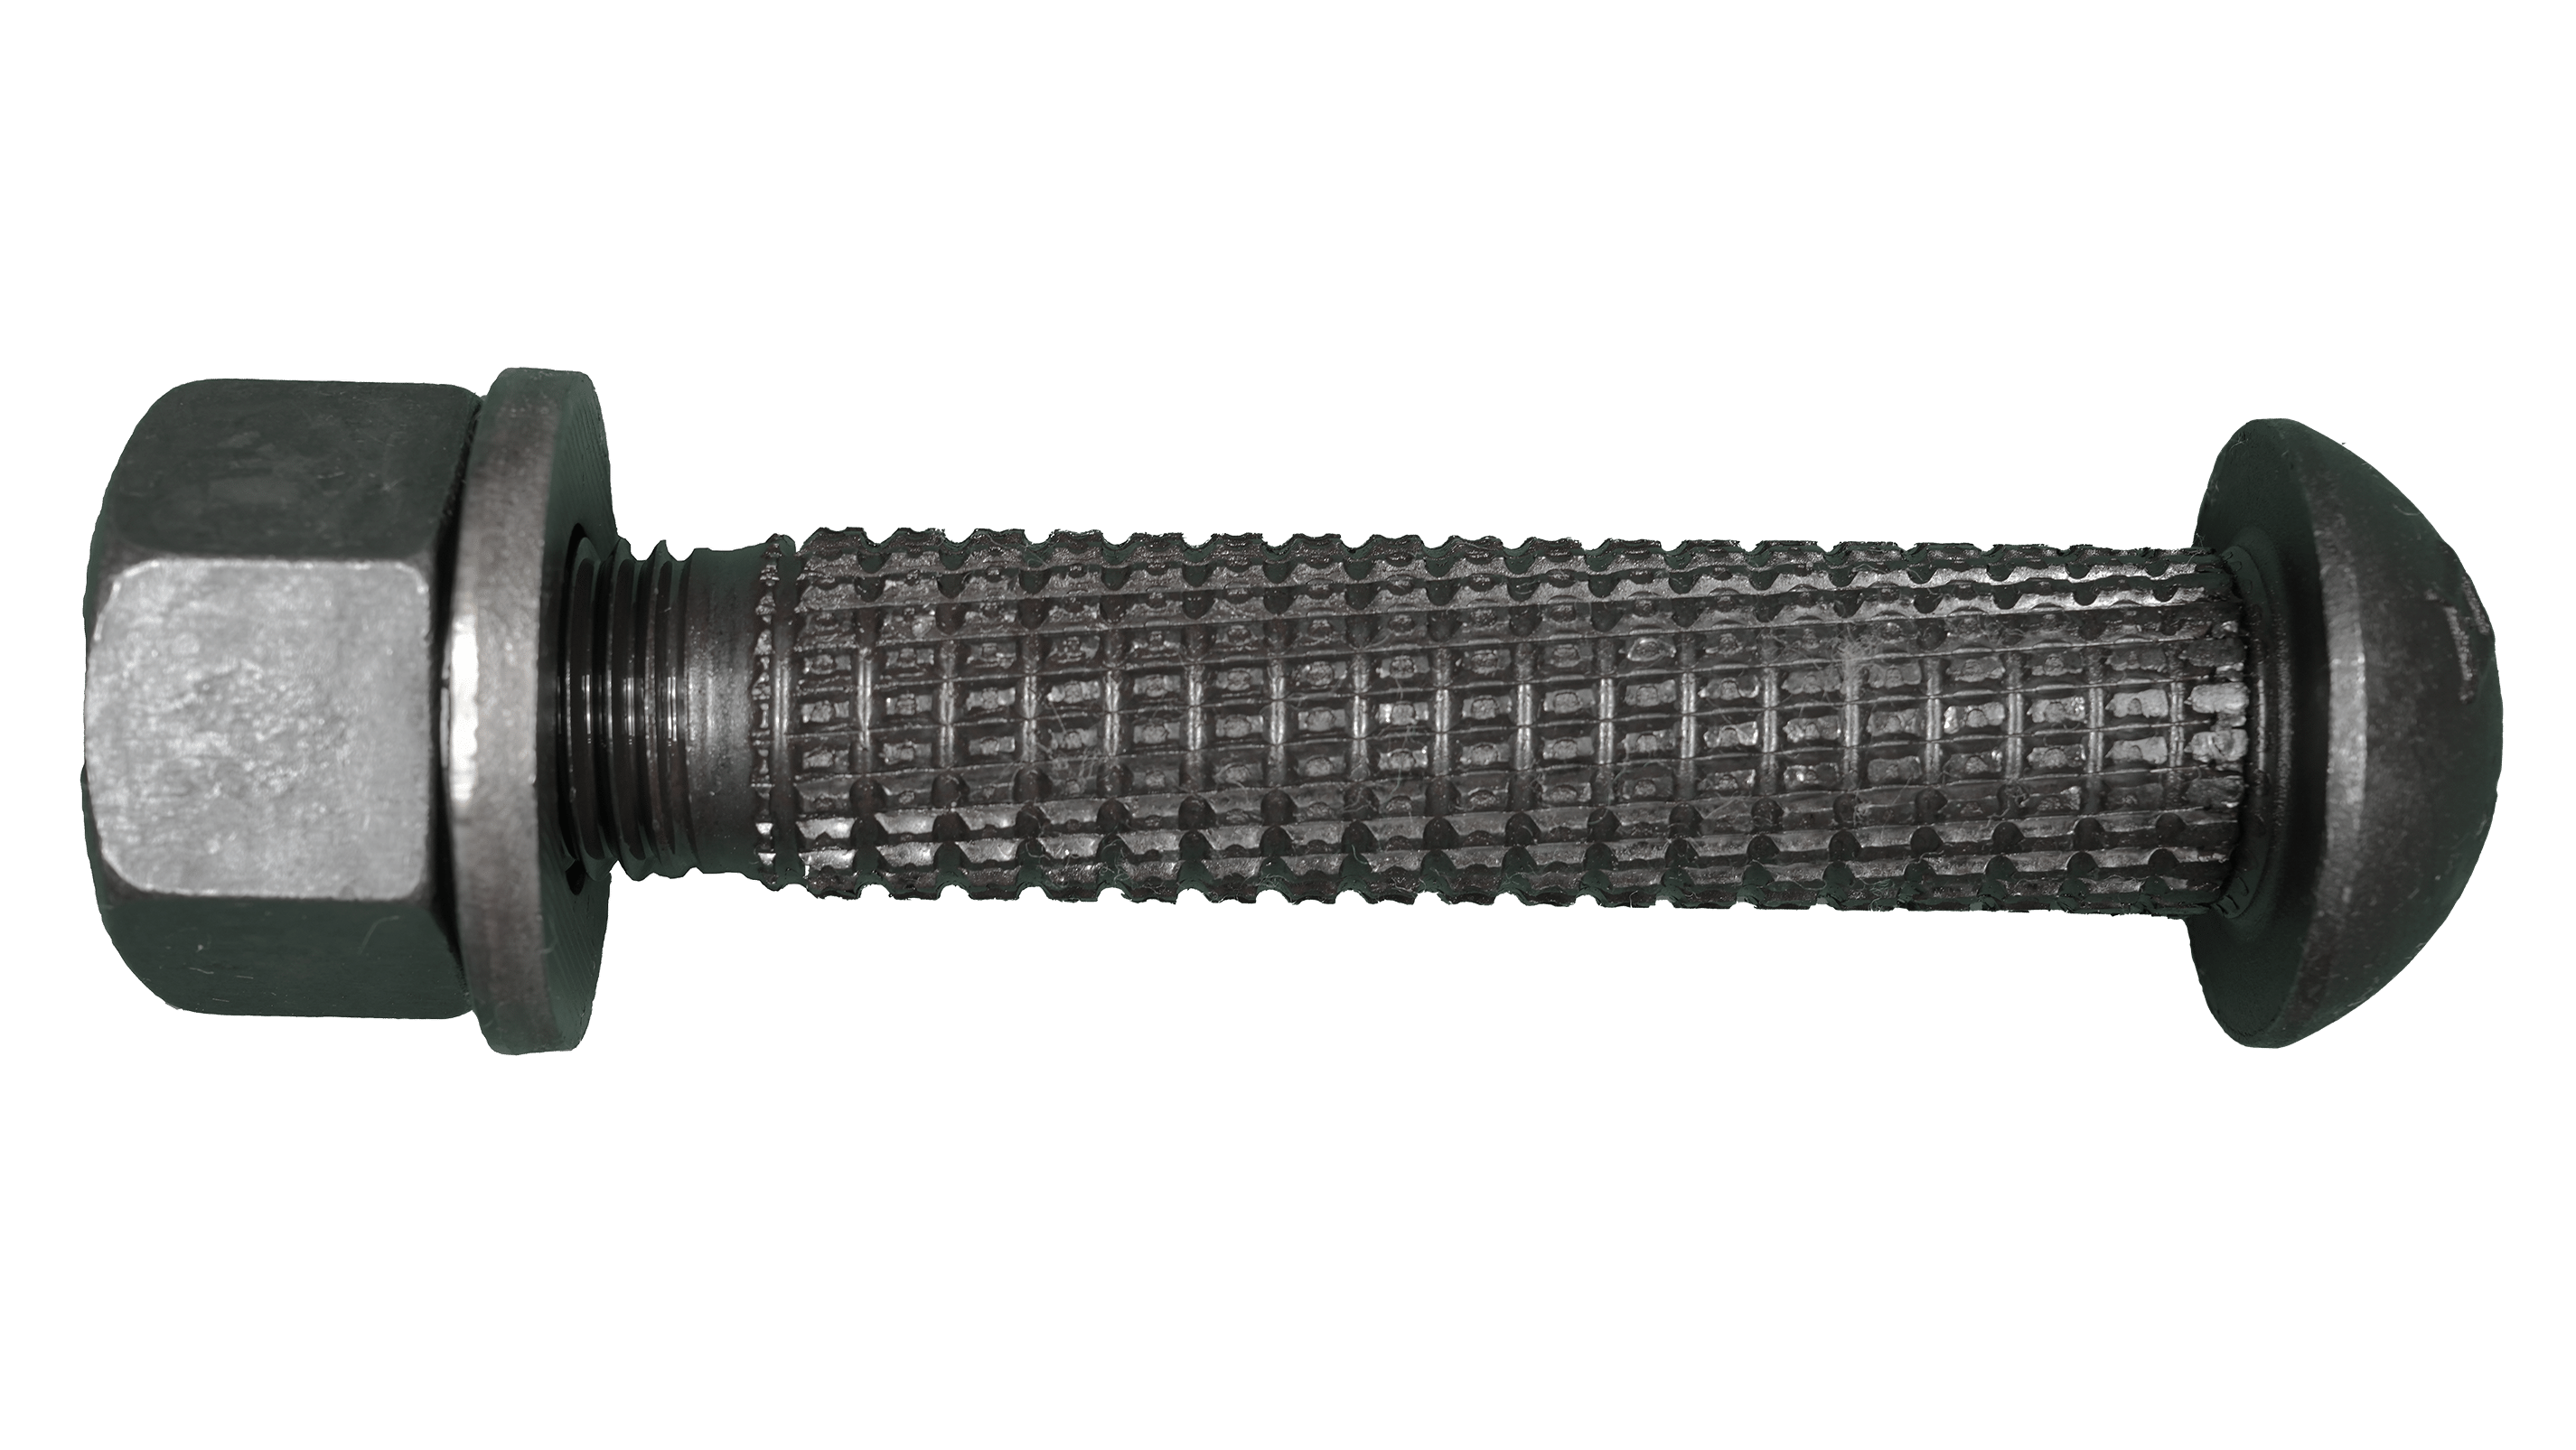
\includegraphics[width=0.7\linewidth]{imgs/ch2/oneBbolt.png}
    \caption{Bearing-type Inteference fit bolt (M22, Diameter = 23.5mm), Made in Kobelco Bolt, Ltd.}
    \label{fig-onebbolt}
\end{figure}

Fig.\ref{fig-cs-b1} shows the cross-sectional diagram of the inteference fit bolt, The cross-sectional diagram was obtained from the hybrid joint that underwent a load of up to 1800kN. Revealing that the deformation of the rib on the non-bearing side is very small as observed in the magnified portion of bolt \#1 on the right side. It has been discovered that despite accurately drilled bolt holes, the interference fit of the rib is not behaving as expected, resulting in a small gap that directly impacts load transfer efficiency. The method of interference fit requires further exploration.

\begin{figure}
    \centering
    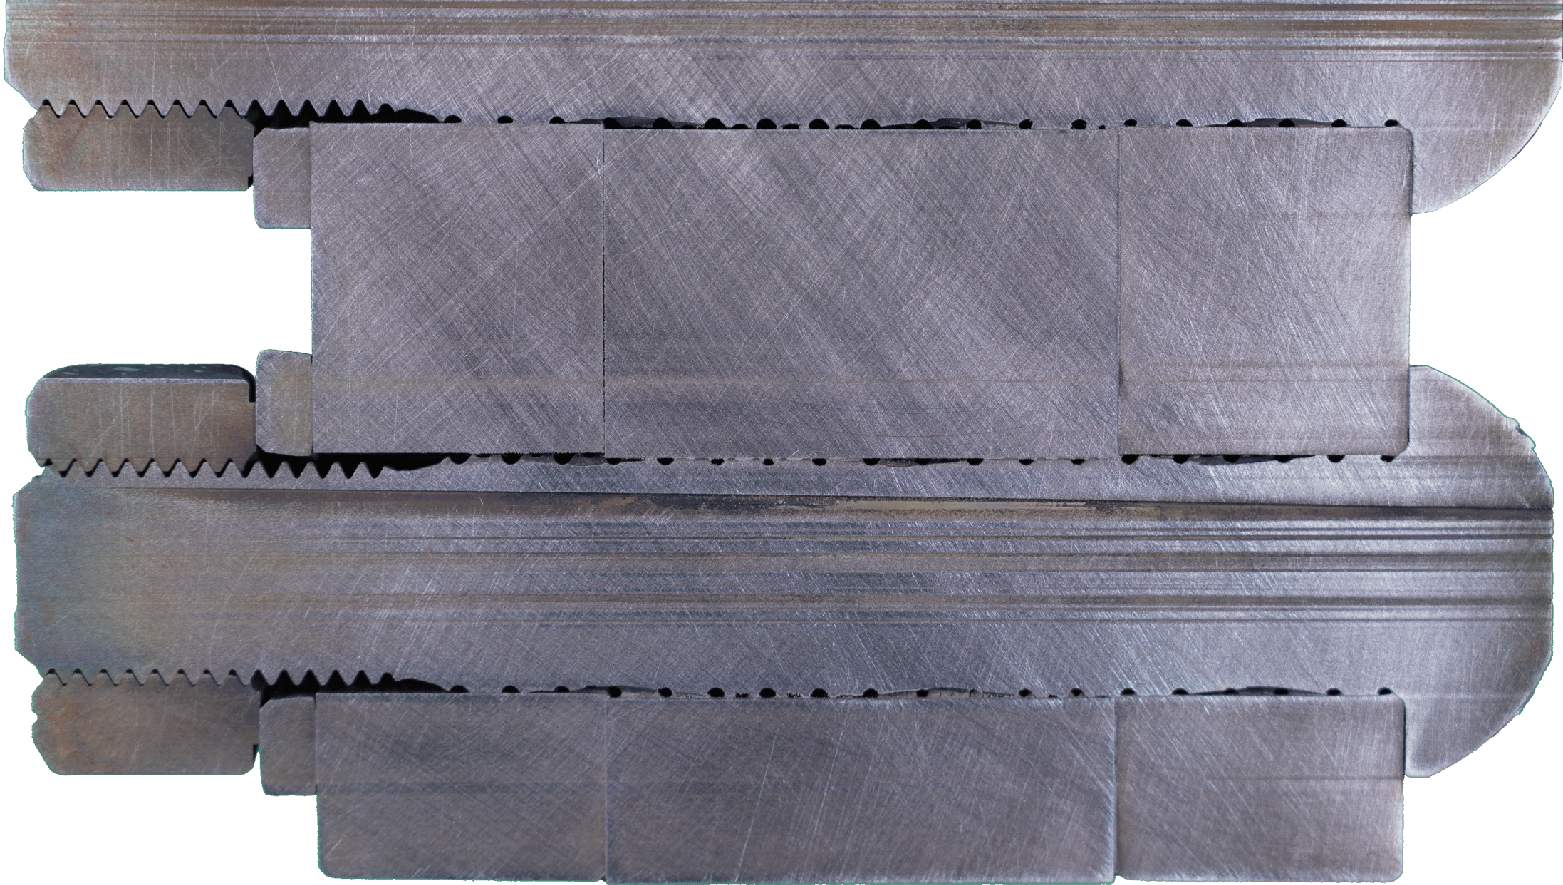
\includegraphics[width=0.8\linewidth]{imgs/ch2/cs-b1.pdf}
    \caption{Sawed-throug cross-section view of interference fit bolt}
    \label{fig-cs-b1}
\end{figure}

Eurocode 3 state that the fit bolt should be desgined using the same methods as the normal High strength bolt,
CSSS consider the bearing resistance of the fit bolt could be expected, the fit bolt also could be using slip resistance designed as the serviceability limit state.

In the JSHB, there only have bearing type connection design methods, but not for interference fit bot, for more effectively use this bolt to provide higher resistance.


\subsection{Resin injected bolt}

Resin-injected bolts are fasteners in which the gap created by the clearance between the bolt and the wall of the hole is filled with a two-component resin as shown in \ref{fig-resinbolt}. They are an effective alternative for bolts fitted with high-strength friction grip bolts in shear connections where slip is not allowed. Injection bolts are a reliable and relatively low-cost option for repairing and improving existing structures \cite{gresnigt1996injbolt}. They are also being used successfully in constructing new structures. The clearance of an injection bolt is filled via a small hole in its head. Once the resin injection is complete and cures completely, the connection becomes slip-resistant. Bearing and shear of the bolt transfer the shear load. In addition, standard structural bolts can be used to fabricate injection bolts. The bolts and washers have been modified to facilitate the injection of resin. The recommendations of ECCS and the Eurocode3 \cite{eurocode3-21,EN14399}for executing steel structures establish the design and execution regulations for injection bolts.

This particular bolt is utilized and analyzed in Europe \cite{pedrosa2022injbolt-mec,kolstein2017injbolt-mec,pedrosa2020injbolt-fati,pedrosa2021injbolt-fati,gresnigt2000injtbolt-use,ungermann2023injbolt-mec}; however, there is no examination or usage of it in Asia. A small quantity of research exists regarding this bolt type within Japan \cite{fujino2010resbolt,Ryota2018resbolt}.

\begin{figure}[htbp]
    \centering
    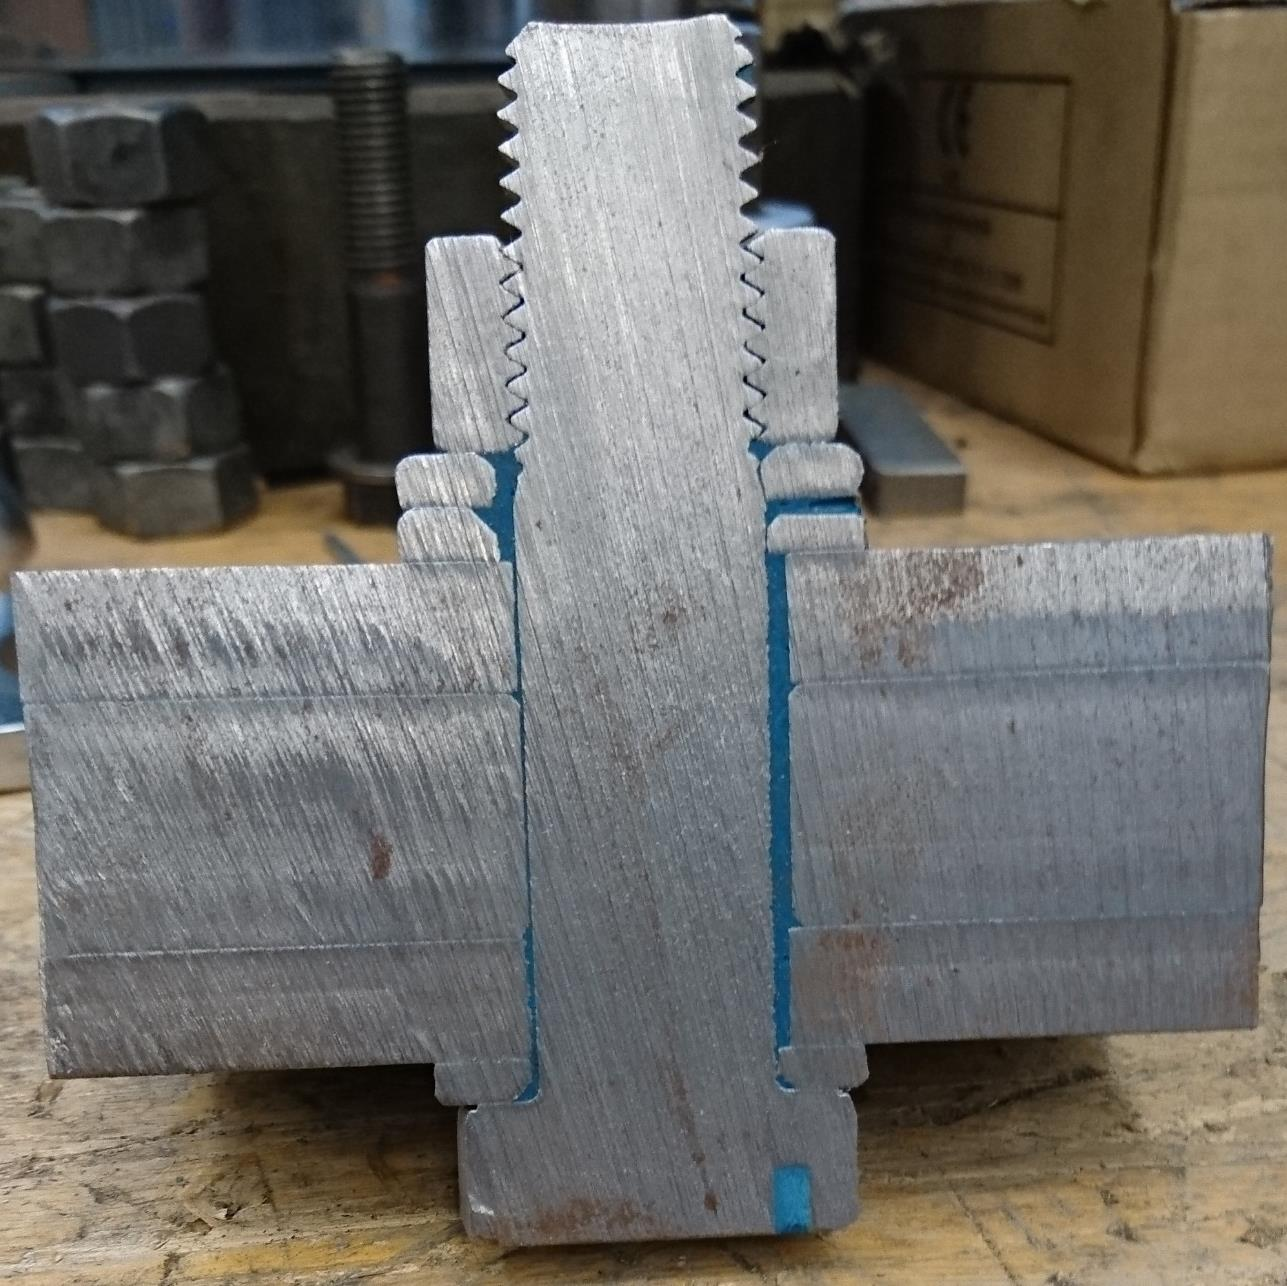
\includegraphics[width=0.65\linewidth]{imgs//ch2/resin-bolt.jpg}
    \caption{Sawed-through (resin) injection bolt connection \cite{Axel2017injbolt}}
    \label{fig-resinbolt}
\end{figure}

\subsubsection{resistance for the resin injection bolt}

For the resin injection bolt, Eurocode 3 state that the strength could be calclutated by sum of 
bearing resistance for the resin and the slip resistance. Although this equation still should be improve, because the resistance between slip and bearing could not simply add, such as the effect of load sharing.


\begin{equation}
    F_{Rd,ser,EC3}=F_s+F_{b,resin}
\end{equation}   

The bearing resistance of resin shall taken as:

\begin{equation}
    F_{b,resin}=\beta dt_{b,resin}f_{b,resin}
\end{equation}

where, $\beta$ is a coefficient depending on the thickness ratio of the main plates. $t_{b,resin}$ is the effective bearing thickness of the resin. 

%todo why the bearing area of resin should be consider the effective area.

\subsection{Other: Mechanical bearing blind rivet-bolt}

The above two types of bolted connections have been used in actual steel construction, in addition to these two types of connection, this year Nakamoto et al. (2022) \cite{Nakamoto2022MBBRB} also proposed the \ac{MBBRB}, which can be installed on one side and transmits the load through the bearing force between the bolt and the wall of the bolt hole, as well as the friction force on the joint surface as shown in Figure \ref{fig-MBBRB}. The load-displacement relationship of the \ac{MBBRB} is equivalent to that of the frictional joint using M22F8T up to the slip load. Therefore, the same service limit state can be applied to the MBBRB joint as to the frictional joint.


\begin{figure}
    \centering
    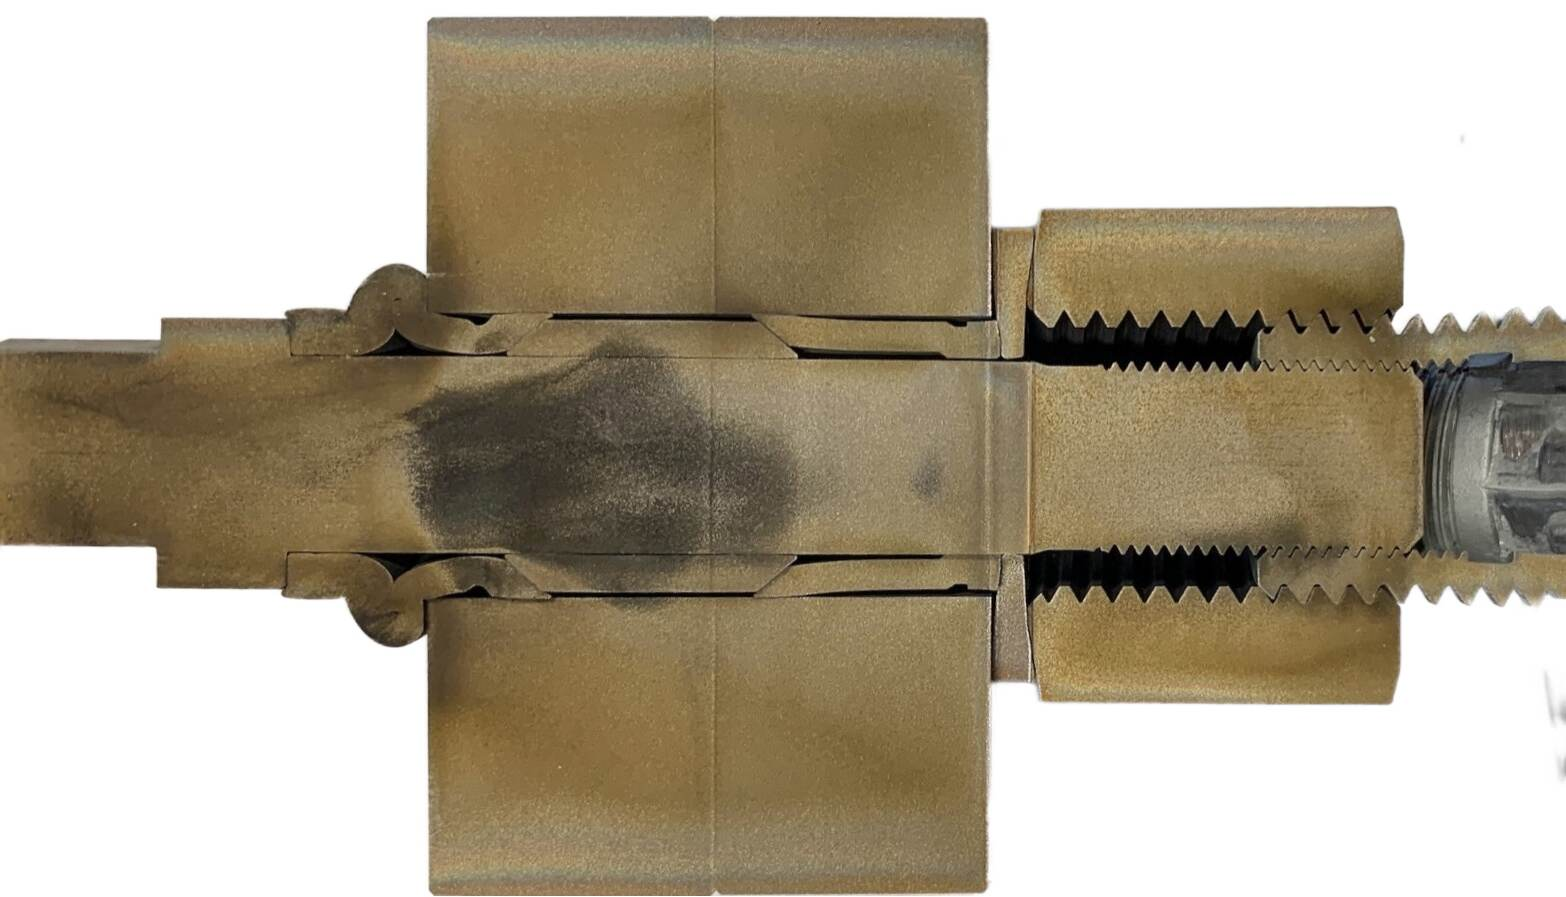
\includegraphics[width=0.85\linewidth]{imgs//ch2/onesidebearingbolt.jpg}
    \caption{Cross-section view of Mechanical Bearing Blind Rivet-Bolts}
    \label{fig-MBBRB}
\end{figure}



\section{Hybrid joint}

Joints are usually made of the same type of fastener, however, in some cases two fasteners with different load transmission mechanisms are assembled on the same joint, which is often referred to as a combination joint or hybrid joint.

The earliest research into hybrid joint was carried out after 1950, when high-strength bolts and welding technology became available as shown in Fig. \ref{fig-schehyb}. Due to the deterioration of riveted bridges, repair work was carried out on riveted connections, and high-strength bolts with better structural performance became one of the alternatives, but the prevailing view at the time was that connections with different mechanical load transfer mechanisms should not be combined, and, in addition, the prevailing research focused on discussing the performance of high-strength bolts and welds.

\begin{figure}[ht]
    \centering
    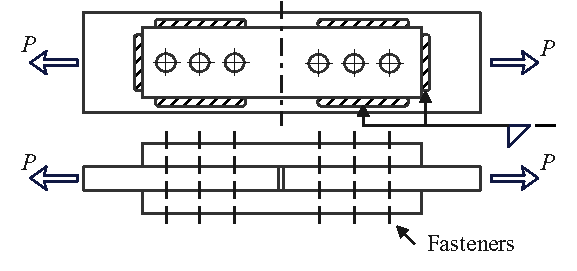
\includegraphics[width=0.75\linewidth]{imgs//ch2/hybrid-sche.pdf}
    \caption{Schematic diagram of Double cover butt hybrid joint (Welding-fasteners)}
    \label{fig-schehyb}
\end{figure}

\subsection{Example of application of hybrid joint}

Aging rivets need to be replaced due to factors such as corrosion of the rivet head and loosening of rivets caused by repeated loading. Despite the requirement for repairs and maintenance of riveted bridges, replacement of original rivets with new ones is not preferred due to the loss of riveting technology and poor constructability of the rivets. In Japan, the use of HSB to replace rivets and form hybrid joints is a common method. Although there are numerous issues that need to be addressed, such as determining the reliability of the slip coefficient of the faying surface and clarifying the mechanism of load transmission. Fig.\ref{fig-bridrivhsb} shows a riveted bridge that is undergoing repair with a mixture of rivets and high-strength bolts. Generally, the original rivets will be removed first, and depending on the situation, it will be chosen whether to replace the cover plate or not, and if necessary, some simple sandblasting and grinding will be performed on the connection surface in order to improve the slip coefficient of the connection surface, and finally the installation of high-strength bolts will be carried out.

%
\begin{figure}[ht]
    \centering
    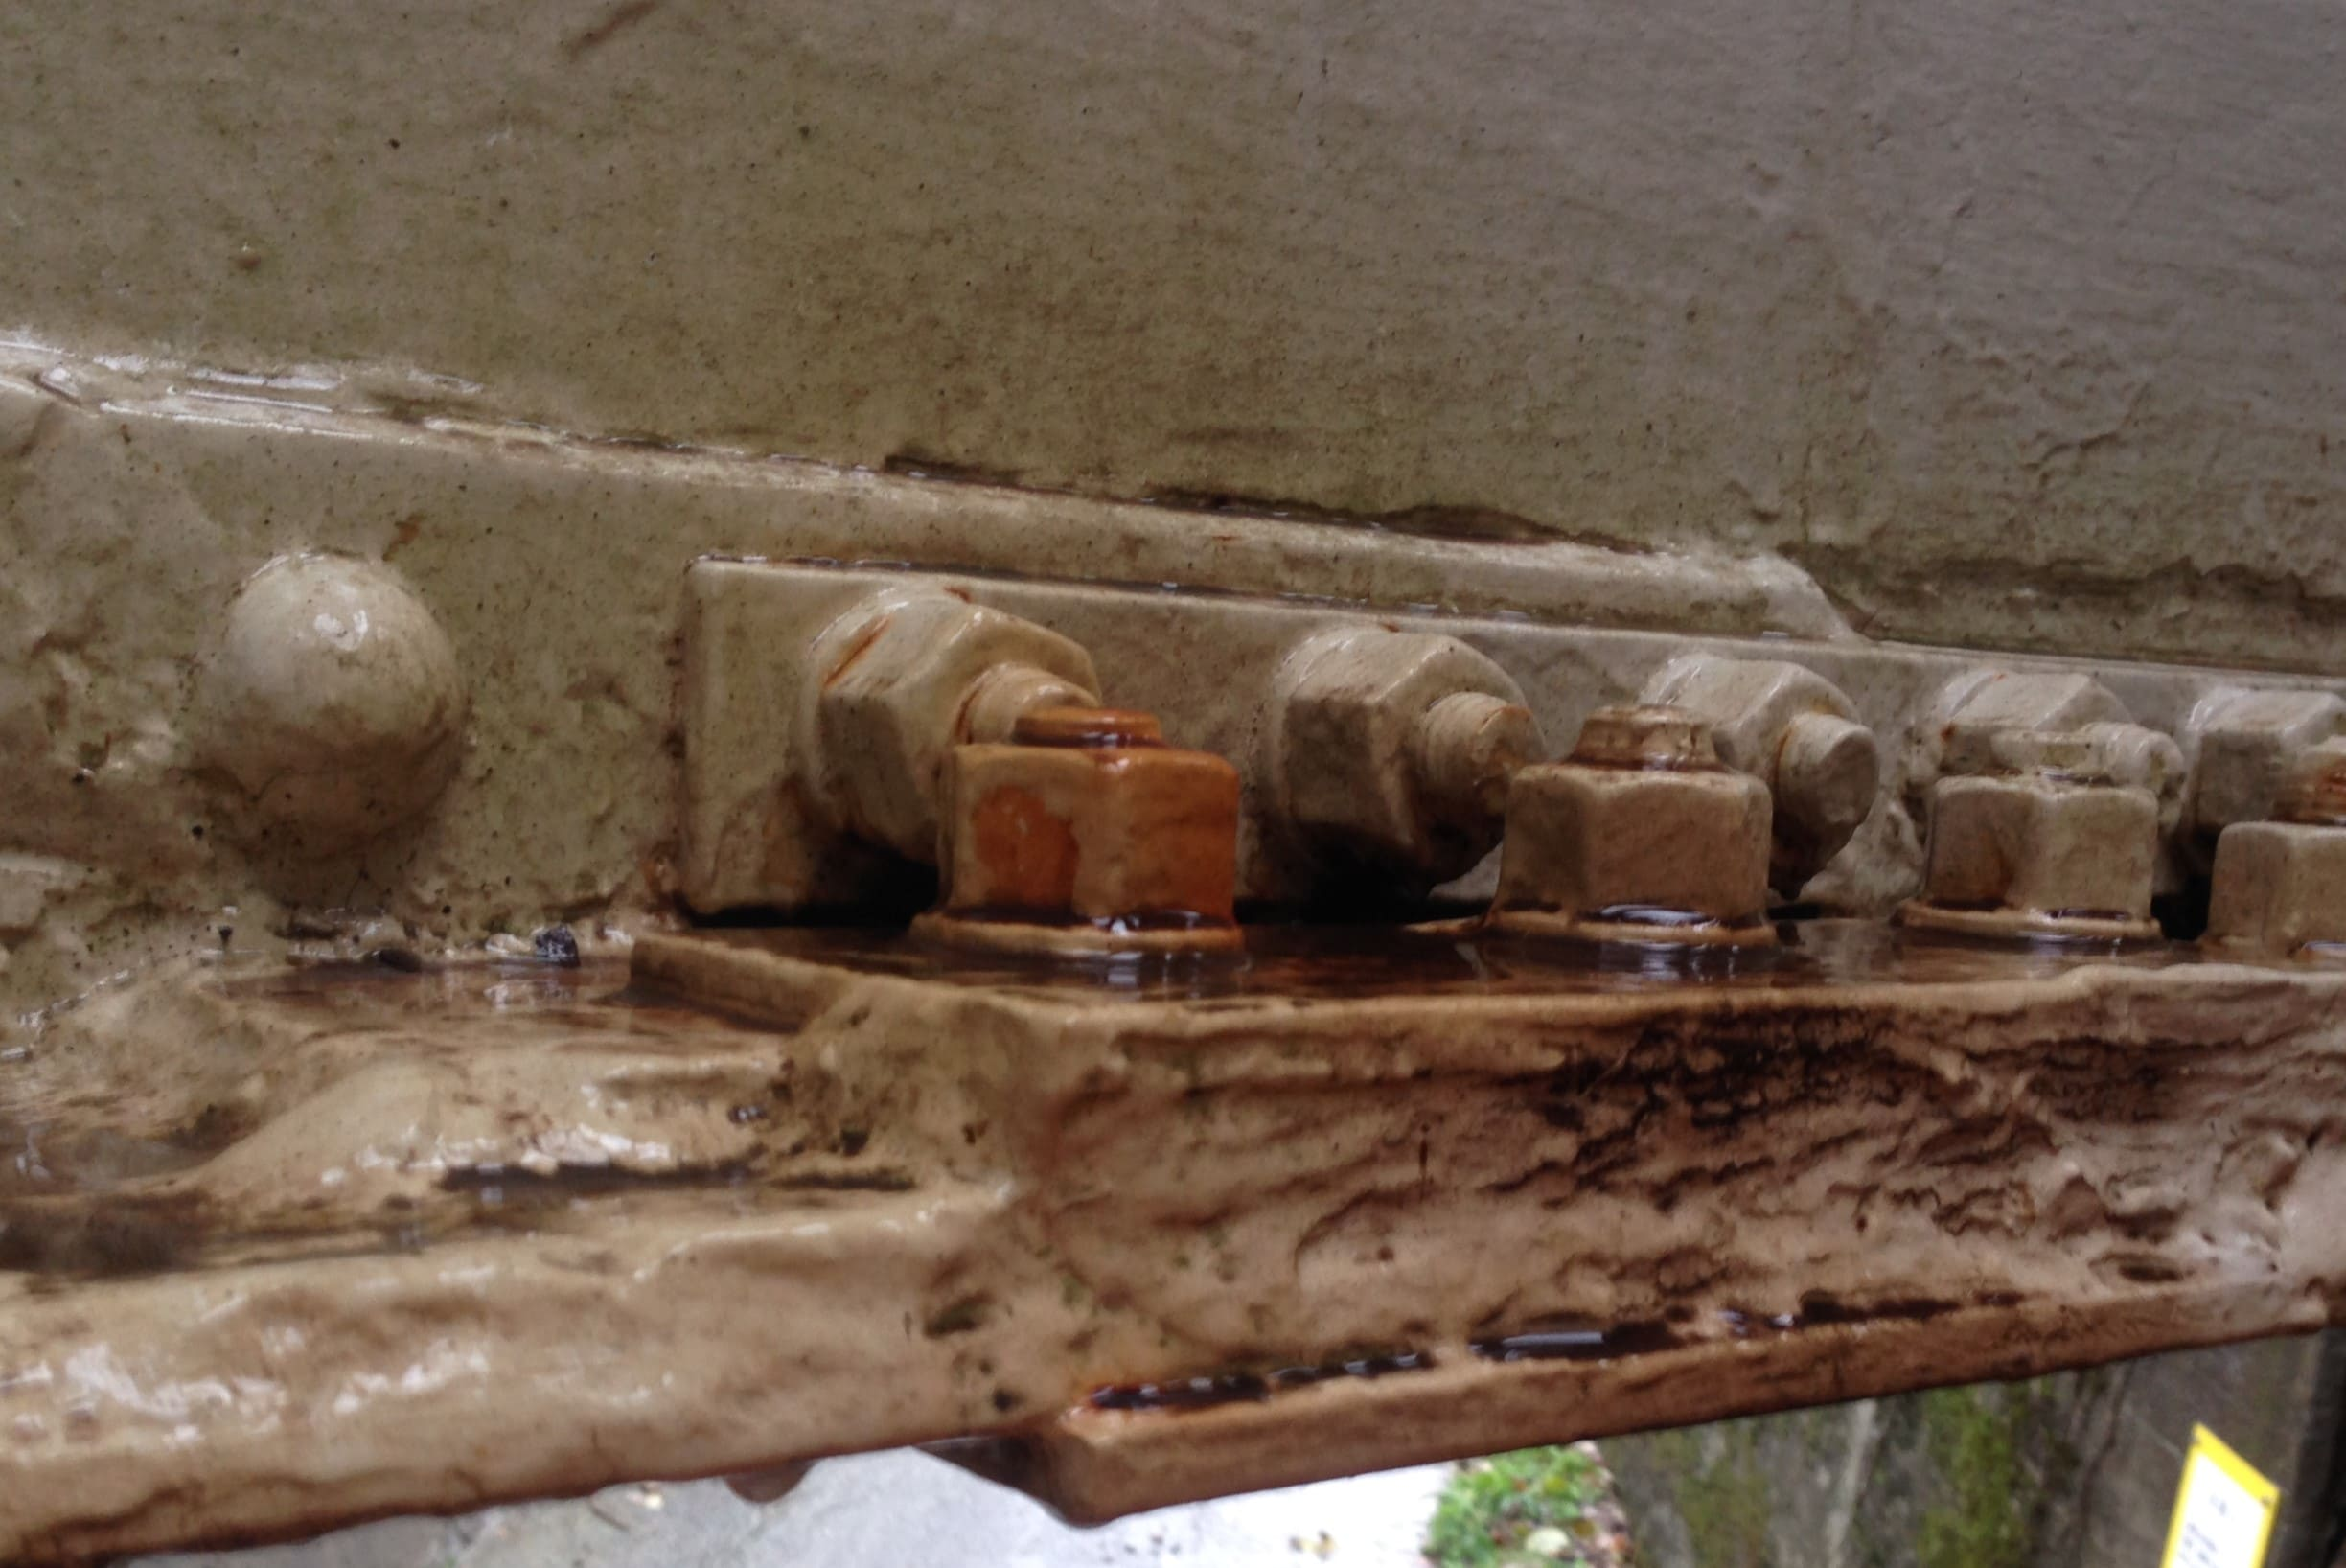
\includegraphics[width=0.75\linewidth]{imgs//ch2/bridge-rivet-HSB.jpg}
    \caption{Riveted joint combined with high-strength bolts. (Hazukawa riveted bridge, Fukui, Japan)}
    \label{fig-bridrivhsb}
\end{figure}

On the other hand, interference fits bolt are also being examined as an alternative to rivets. Substituting the rivets with fasteners that are also transmit load by bearing would have been a more practical option. However, there have a serious problem is that when drilling out the rivets, the original rivet holes have to be slightly enlarged, making it difficult for the IFBs to produce an interference fit effectively. Additionally, due to the precision requirements of the IF bolts, it is challenging to employ them as substitutes for the rivets in fact engineering.

When replacing rivets, it may be necessary to adjust the length of the joint to accommodate the possible addition of extra bolts to enhance its strength. However, the limited space within the bridge girder and the geometry of its components may render the installation of additional bolts impossible, the use of welds to increase the strength of the joint is usually considered in this case \cite{Thomas2000}.

For riveted and welded joints, Bryla(1932)\cite{bryla1932Tests} conducted the first test of hybrid riveted and welded joints but considered only the ultimate strength of the joints. Consideration of riveted and welded fits from the point of view of ultimate strength only does not establish a factor of safety for the strength of the joints. More studies on load distribution followed by Sakurai(1951) \cite{sakurai1951Experimental}, discussing the effects of the construction sequence of riveted and welded joints as well as of the coefficients of the load distribution of riveted and welded joints.

Welding and riveting can share a significant amount of load if handled properly, and the weld has sufficient stiffness and strength to transfer loads other than those originally shared by the rivet, and this type of reinforcement is considered effective \cite{young1934Relative,hiroshi2001Experimental,meier2000composite}. However, the reality is that in the case of old riveted bridges, the steel of the time contained more impurities, i.e. the steel of old riveted bridges is not suitable for welding, and due to the corrosion that often accompanies it, it is difficult to carry out high quality welding work in the field, which directly affects the tensile and fatigue strength of the weld, and therefore welding is not recommended for strengthening riveted bridges, except in special circumstances.

\subsection{Rivet-HSB}

The incorporation of high-strength bolts into a riveted connection yields various enhancements. In terms of a specific diameter, a high-strength bolt demonstrates superior shear strength compared to a rivet, thereby leading to an overall increase in the ultimate strength of the entire connection. Additionally, the inclusion of high-strength bolts contributes to an augmented stiffness in slip-resistant connections. In the event that slip resistance is surpassed, the presence of rivets, which possess narrower hole clearances relative to high-strength bolts, restricts the occurrence of slip in relation to a fully-bolted joint. Furthermore, research has substantiated that substituting rivets with high-strength bolts enhances the fatigue strength of the joint \cite{reemsnyder1975Fatigue}.

\subsubsection{Mechanical behavior}

Experiments conducted to assess the load-deformation characteristics of short bolted-riveted hybrid joints have revealed that the total resistance offered by the joint can be adequately estimated by summing up the individual resistances provided by the two different types of fasteners.

Komatsu et al.\cite{KOMATSU2015} conducted tensile load tests and chemical tests on aged steel to understand its fundamental properties. Furthermore, tensile loading tests were performed on multi-bolted joints to investigate the replacement of rivets with HSB. The test results reveal that the load carrying capacity and deformability of the partially and fully replaced HSB. joints can be enhanced by introducing frictional resistance, compared to riveted joints alone.

Fig.\ref{fig-hsbriv-fune} \cite{funahashi1967Experimental} and Fig.\ref{fig-hsbriv-stei} \cite{steinhardt1969-hybrid} show typical load versus deformation curves for welded, bolted, and riveted tension specimens. This figure indicates that high-strength bolted connections with normal hole clearance provide a very high initial stiffness up to the slip load of the connection. During slip, the deformations increase significantly until the bolts come into bearing. After the bolts are in bearing, the load versus deformation curve shows an increase in joint stiffness. Joint slip can be minimized by installing fitted bolts in matching drilled holes.

\begin{figure}
    \centering
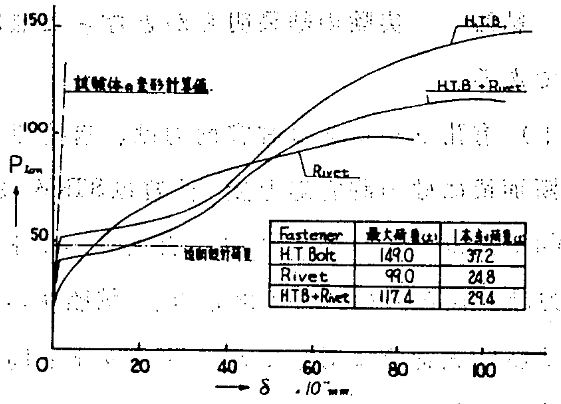
\includegraphics[width=0.75\linewidth]{imgs//ch2/hsbrivet-1967-pd.png}
    \caption{Relationship between load and deformation of Hybrid joint combined with 2 HSB and 2 rivet \cite{funahashi1967Experimental}}
    \label{fig-hsbriv-fune}
\end{figure}

\begin{figure}
    \centering
    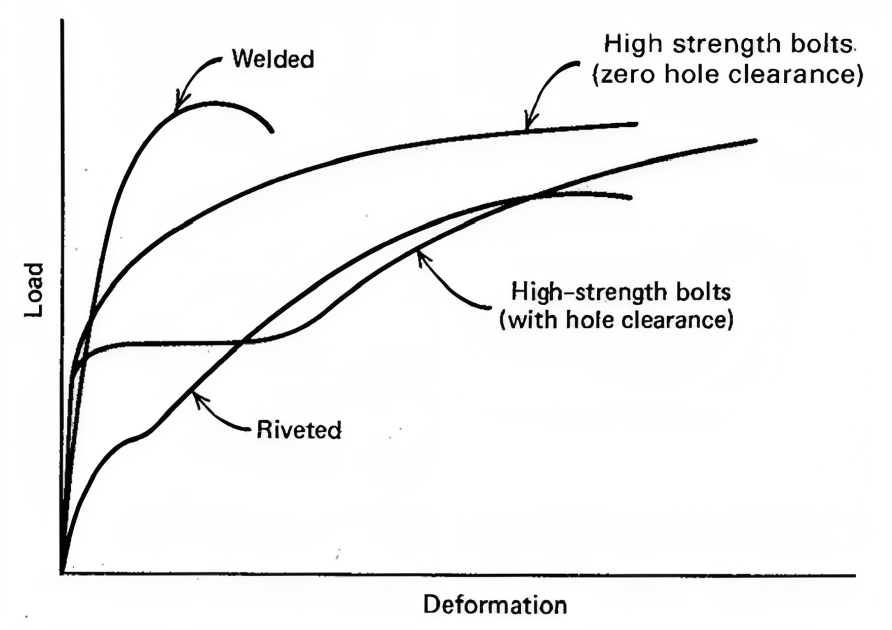
\includegraphics[width=0.75\linewidth]{imgs//ch2/hsbrive-1969.png}
    \caption{Load versus deformation relationships for different fastening methods \cite{steinhardt1969-hybrid}}
    \label{fig-hsbriv-stei}
\end{figure}


One limitation of high-strength bolted connections is their decreased deformation capacity. Welded connections do not experience slip, and the initial stiffness of the joint remains relatively constant until the ultimate load is reached. Based on the load-deformation relationships observed in typical fasteners, it can be inferred that the most suitable combination of fasteners is one that possesses compatible deformation characteristics. In this regard, the preferred combinations seem to be welds in conjunction with slip-resistant high-strength bolts, as well as rivets alongside bolts.

Given that the joint strength of short combination joints is a sum of the strengths of individual fasteners, the specific arrangement of these fasteners within the combination joint becomes inconsequential. Consequently, both the outermost rivets and the rivets within the joint can be interchanged with high-strength bolts, as either arrangement results in a similar ultimate load. However, it should be noted that the location of fasteners does influence the joint strength, as observed in long riveted and bolted joints. In the case of long joints, the replacement of outermost rivets with high-strength bolts proves more effective in enhancing joint strength than replacing the same number of interior fasteners, primarily due to the phenomenon of "unbuttoning." The location of the bolts as well as the rivets configuration will be studied and explored as part of the research objectives of this study.

\subsubsection{Fatigue strength}

The research findings \cite{steinhardt1969-hybrid, reemsnyder1975Fatigue} demonstrated that substituting rivets with preloaded high-strength bolts in areas where cracking was observed or anticipated resulted in a fatigue life improvement ranging from two to six times. It is imperative to ensure the careful extraction of the rivets to be replaced and the accurate installation of the replacement bolts during the rehabilitation process to prevent the introduction of new mechanical flaws, such as burrs, nicks, and gouges. Furthermore, the tests indicated that if cracking is mitigated in the crucial region through rivet replacement, other less highly stressed areas may then become susceptible to becoming critical.


\subsection{HSB-Weld} \label{sec-hsbweld}

Adding Welds to Mechanically Fastened Joints Welded connections are rigid. Welded connections are stiff. Unlike snug-tightened bolted joints that may slip as they are loaded, welds are not expected to stretch and distribute the applied load to any great extent. In most cases, welds and bearing-type mechanical fasteners will not deform equally.

When welds and mechanical fasteners are used together, load is transferred through the stiffer part; therefore, the weld can carry almost all the load, sharing little with the bolts. That is why caution needs to be taken when welds, bolts, and rivets are combined.Code Provisions. The issue of mixing mechanical fasteners and welds is addressed in AWS D1. 1:2000 Structural Welding Code—Steel \cite{aws2000AWS}. Provision 2.6.3 states that for rivets or bolts used in bearing-type connections (that is, when the bolt or rivet acts as a pin), the mechanical fasteners should not be considered as sharing the load in combination with welds. If welds are used, they should be provided to carry the entire load in the connection. However, connections that are welded to one member and riveted or bolted to another are permitted.


Holtz and Kulak (1970) \cite{holtz1970high} carried out a series of tests on combination joints. In these experiments, a double lap joint featuring both bolts and welds in the same shear plane was subjected to tension loading. They found that bolts carry only a limited amount of load at service loads (considered to be around 1/3 of ultimate load). They also observed that it is unreliable to predict the impact of friction when using pretensioned bolts. Moreover, bolts do not perform efficiently when combined with transverse welds due to the latter's limited ductility.



%https://www.thefabricator.com/thefabricator/article/arcwelding/mixing-welds--bolts
%https://pressbooks.bccampus.ca/powr4406/chapter/bolted-and-welded-joints/

\subsection{IFB-HSB}


\section{Summarize for the issue of hybrid joint}

During the reconstruction projects following the Second World War, the combined use of diverse connection methods with varying principles presented challenges. For instance, when reinforcing aging riveted structures by welding or partially replacing them with \ac{HSB}, difficulties arose. Joining components with combined different load transfer mechanism connection methods results in a non-stationary structure, making it difficult to accurately calculate the sharing of loads in the past. As a result, only one of the two types was considered valid for design purposes at the time, denying the cooperative actions expected from their combined use.

The maintenance and repair of ageing riveted bridges is expected to face increasing challenges from now on. Bridges must achieve a compromise between suitable flexibility and rigidity. The addition of reinforcing elements to a completed bridge may upset this equilibrium and create problems. Consequently, post-construction reinforcement of a bridge may present a challenge by using hybrid connection.

In addition, for new structural components, the rational use of hybrid joints can effectively improve the strength of the joints and shorten the length of the joints as much as possible, while meeting the required strength to make the joint compact.  However, unlike the reinforcement of an existing structural component, new structural components raise issues of structural stability, durability and strict requirements for allowable deformation, and require a series of tests before they can be installed.

In summary, this work focuses on the following technical issues:

\begin{itemize}
    \item The primary technical challenge lies in the lack of understanding regarding the load transfer mechanism when combining connections with different mechanical principles.
    \item To use hybrid joints effectively, it is essential to comprehend not only how the load gets transferred but also the optimal arrangement of fasteners. Different arrangements may produce different load transfer effects, so exploring the reasonable fastener arrangement scheme will be an important technical problem.
    \item The stiffness of Friction connection and bearing connection are different. In the case of a friction connection, there will be a small elastic dislocation (slip) before occurrence, which is a different mechanical mechanism from the elastic deformation of a bearing connection. Exploring the deformation capacity of the bearing and friction combination is also an important technical subject.
    \item After understanding the load transfer mechanism, strength and deformation performance of hybrid connections, it is necessary to define their limit states and to devise how to differentiate between the limit states and their corresponding strength equations.
    
\end{itemize}

% \section{Regulations and standards}

% \subsection{Riveted joint}

% Shear resistance, per shear plane, Eurocode:
% \begin{equation}
% F_{\mathrm{v}, \mathrm{Rd}}=\frac{0,6 f_{\mathrm{ur}} A_0}{\gamma_{\mathrm{M} 2}}
% \end{equation}